\PassOptionsToPackage{table}{xcolor}
\documentclass[9pt,twocolumn]{extarticle}
\usepackage[a4paper,margin=14mm,top=16mm,bottom=16mm,columnsep=7mm]{geometry}
\usepackage[T1]{fontenc}
\usepackage[utf8]{inputenc}
\usepackage[scaled=0.92]{helvet}
\renewcommand{\familydefault}{\sfdefault}
\usepackage{needspace}
\usepackage{graphicx,float,booktabs,tabularx,array,amsmath,microtype,titlesec,caption,tcolorbox,longtable}
\usepackage[table]{xcolor}
\usepackage[hidelinks]{hyperref}
\usepackage[round]{natbib}
\definecolor{sky}{HTML}{2F6FBA}
\definecolor{dusk}{HTML}{C8562B}
\definecolor{ink}{HTML}{1C2230}
\definecolor{rowa}{HTML}{EEF2F7}
\titleformat{\section}{\Large\bfseries\color{sky}}{}{0pt}{}[\vspace{-6pt}{\color{sky}\rule{\linewidth}{0.6pt}}]
\titleformat{\subsection}{\normalsize\bfseries\color{ink}}{}{0pt}{}
\titlespacing{\section}{0pt}{10pt}{6pt}
\titlespacing{\subsection}{0pt}{8pt}{3pt}
\captionsetup{font={footnotesize,sf},labelfont={bf,color=sky},justification=raggedright,singlelinecheck=false,skip=3pt}
\setlength{\parskip}{3pt}\setlength{\parindent}{0pt}
\raggedbottom
\newcolumntype{Y}{>{\raggedright\arraybackslash}X}
\renewcommand{\arraystretch}{1.15}
\setlength{\tabcolsep}{4pt}

\begin{document}
\twocolumn[
\begin{@twocolumnfalse}
\vspace*{-6mm}
{\color{sky}\fontsize{28}{30}\selectfont\bfseries The color of Earth's sky,\\ 4.4 billion years to today\par}
\vspace{6pt}
{\large\color{ink} What the sky looked like from the ground---straight up and at the horizon, at the equator and the poles, at noon and at dusk---at eighteen moments in Earth's history, reconstructed with a spectral radiative-transfer model; and the rest of its sky, from the green flash and the eclipsed Moon to airglow, aurorae and meteors.\par}
\vspace{4pt}
{\small\color{gray} Prepared with Claude (Anthropic) $\cdot$ October 2026\par}
\vspace{8pt}
{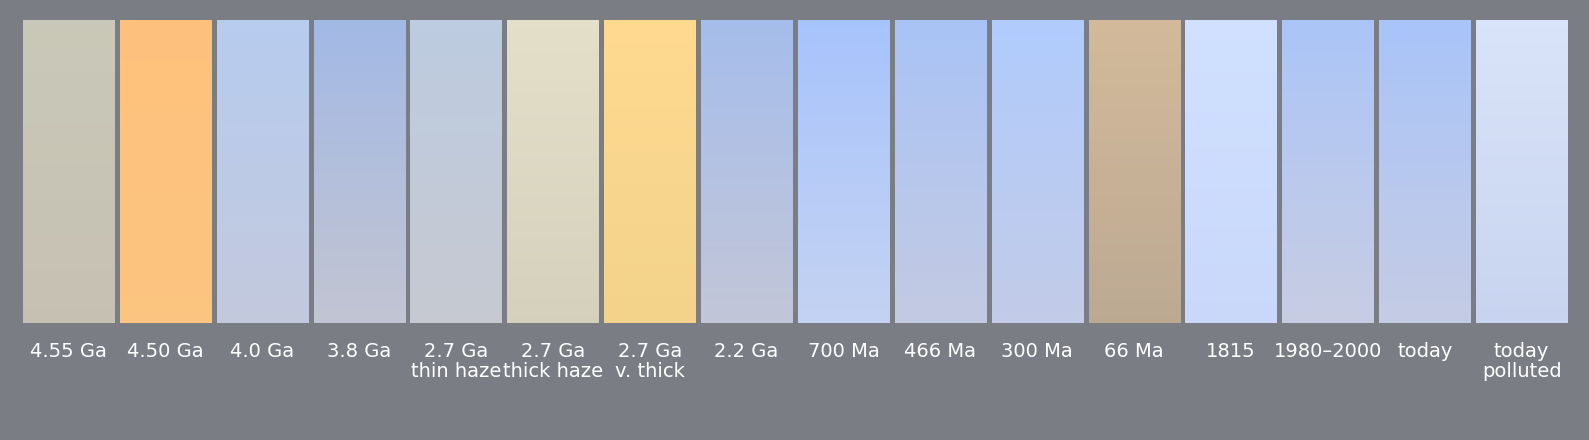
\includegraphics[width=\linewidth]{figures/fig01_timeline.png}}
{\footnotesize\sffamily\textbf{\color{sky}Figure 1.} Mid-latitude noon sky at fifteen epochs, zenith (top) to horizon (bottom), oldest at left. Brightness shown relative to today's clean sky.\par}
\vspace{10pt}
\end{@twocolumnfalse}
]
\setcounter{figure}{1}

\begin{tcolorbox}[colback=rowa,colframe=sky,boxrule=0.6pt,arc=1.5pt,left=5pt,right=5pt,top=4pt,bottom=4pt,title=\textbf{Seven things the sky did},fonttitle=\bfseries]
\footnotesize
\textbf{1.} Under the 30-bar CO$_2$ atmosphere of the early Hadean the sky was a shadowless peach-white glow with no visible Sun.\\
\textbf{2.} During the hazy Neoarchean the whole dome was cream to apricot, with almost no difference between zenith and horizon.\\
\textbf{3.} Before the Great Oxidation Event there was no ozone, so every twilight ended in a cream zenith. The first ozone layer turns that zenith pale blue; the deep blue dusk needs a near-modern column.\\
\textbf{4.} Snowball Earth had the bluest sky in Earth's history; the K--Pg impact winter had no sunsets at all.\\
\textbf{5.} The zenith-to-horizon color gradient is the single best diagnostic of an atmosphere's state: largest in clean air, gone under haze or soot, reversed under volcanic sulfate.\\
\textbf{6.} The eclipsed Moon is copper today, orange-rimmed before there was ozone, an even deep red through the Hadean CO$_2$, dark-cored when the Moon was close, and gone under the K--Pg soot, the thick Archean haze or a Tambora veil.\\
\textbf{7.} Before the Great Oxidation the nights were darker and violet: no oxygen airglow, nitrogen aurorae reaching the mid-latitudes, and meteors with no glowing trains.
\end{tcolorbox}

\section*{Has this been done before?}
Not as such. A search of the Valency corpus (arXiv, PubMed, EarthArXiv and others) finds the two halves of the problem solved separately but never joined. On one side, atmospheric-optics work computes modern sky color rigorously: \citet{lynch2005} derive CIE chromaticities of the sky, Sun and distant objects from MODTRAN spectra; \citet{peyvandi2016} simulate 5.6 million daylight spectra with SBDART to map how aerosol and ozone shift sky color; \citet{lee2017} show with Monte Carlo simulation that vivid solar-horizon twilight colors need aerosol while the purest antisolar colors occur in a purely molecular atmosphere. On the other side, paleoatmosphere work constrains composition: \citet{catling2020} for the Archean (O$_2$ below $10^{-6}$ of present, CO$_2$ 10--2,500$\times$ modern, CH$_4$ $10^{2}$--$10^{4}\times$ modern), and \citet{arney2016}, \citet{mak2023} and \citet{goldblatt2024} for the organic-haze episodes. Arney's "Pale Orange Dot" computes what a hazy Archean Earth looks like \emph{from space}, as an exoplanet spectrum, and that is as close as the literature comes. Nobody has computed the view from the ground, or the horizon-versus-zenith, latitude, and sunset structure. So this report does.

\section*{How the colors were computed}
For each epoch the atmosphere is built from components with their own vertical profile and spectral optical depth: Rayleigh-scattering gas (N$_2$, O$_2$, CO$_2$, CH$_4$, H$_2$O in their epoch-appropriate partial pressures), ozone (the Chappuis cross section of Serdyuchenko et al. 2014 at 223 K, on a layer whose peak falls from 26 km at the equator to 18 km at the pole), tropospheric aerosol, a stratospheric sulfate layer, a tholin-like fractal organic haze (strongly blue-absorbing, forward-scattering), and impact soot. Sky radiance is integrated numerically along each line of sight through a spherical-shell atmosphere, so grazing sunlight at twilight is handled properly, with multiple scattering and surface reflection added from a delta-Eddington two-stream solution. The young Sun is treated as a blackbody made fainter and slightly cooler following standard solar evolution: 5,560 K and 70\% of today's luminosity at 4.4 Ga, 5,620 K and 75\% at 3.8 Ga, 5,660 K and 80\% at 2.7 Ga, 5,700 K and 85\% at 2.2 Ga, 5,772 K today. The color effect is only $\sim$200 K, barely perceptible and far smaller than the atmospheric effects; the brightness effect is what makes the early skies dimmer. Spectra from 380--780 nm are converted to CIE XYZ and shown as sRGB. The model reproduces measured modern values (clear zenith 10,000--20,000 K, horizon 6,000--8,500 K, setting Sun $\sim$1,700 K, pink antisolar Belt of Venus) before being pointed backward.

\textbf{The young Sun.} The Sun is treated as a blackbody whose effective temperature and luminosity follow standard solar-evolution tracks: 5,560\,K and 70\% of today's output at 4.4\,Ga, rising through 5,620\,K (75\%) at 3.8\,Ga, 5,660\,K (80\%) at 2.7\,Ga and 5,700\,K (85\%) at 2.2\,Ga to 5,772\,K today (Table~\ref{tab:epochs}). The color effect is small: a 5,560\,K Sun is only about 200\,K cooler in color temperature than the modern one, a difference that is barely perceptible side by side and is swamped by atmospheric effects ten to a hundred times larger. The brightness effect is not small, and is why the early-epoch skies are rendered dimmer. Fraunhofer lines and the young Sun's ultraviolet excess, which matter for haze photochemistry but not for visible color, are ignored.

The model is provided as the Python source \texttt{skymodel.py}; \texttt{run\_epochs.py} produces the sky colors and \texttt{limb\_grid.py} the limb and disk colors for the renderings. Epoch atmospheres are summarized in Table~\ref{tab:epochs}.

\begin{table*}[t]\centering\footnotesize
\caption{Atmospheres used for each epoch. Gas amounts are partial pressures in bar; AOD is tropospheric aerosol optical depth at 550\,nm; haze, sulfate and soot are column optical depths at 550\,nm; $T_{\rm eff}$ and $L_\odot$ are the assumed solar effective temperature and luminosity relative to today.}
\label{tab:epochs}
\rowcolors{2}{rowa}{white}
\begin{tabularx}{\textwidth}{@{}lYrrrrrrr@{}}\toprule
Epoch & Gas (bar) & O$_3$ (DU) & AOD & Haze & Sulfate & Soot & $T_{\rm eff}$ (K) & $L_\odot$ \\ \midrule
4.4 Ga Hadean & CO$_2$ 30, N$_2$ 1, H$_2$O 0.3 & 0 & 0.30 & -- & -- & -- & 5560 & 0.70 \\
4.0 Ga Hadean & N$_2$ 1, CO$_2$ 0.5 & 0 & 0.15 & -- & -- & -- & 5600 & 0.72 \\
3.8 Ga Archean & N$_2$ 0.8, CO$_2$ 0.1, CH$_4$ 0.001 & 0 & 0.08 & -- & -- & -- & 5620 & 0.75 \\
2.7 Ga thin haze & N$_2$ 0.8, CO$_2$ 0.05, CH$_4$ 0.003 & 0 & 0.08 & 0.15 & -- & -- & 5660 & 0.80 \\
2.7 Ga thick haze & N$_2$ 0.8, CO$_2$ 0.05, CH$_4$ 0.005 & 0 & 0.08 & 0.6 & -- & -- & 5660 & 0.80 \\
2.7 Ga very thick haze & N$_2$ 0.8, CO$_2$ 0.05, CH$_4$ 0.01 & 0 & 0.08 & 1.5 & -- & -- & 5660 & 0.80 \\
2.2 Ga post-GOE & N$_2$ 0.8, O$_2$ 0.002, CO$_2$ 0.02 & 66 & 0.10 & -- & -- & -- & 5700 & 0.85 \\
700 Ma Snowball & N$_2$ 0.78, O$_2$ 0.02, CO$_2$ 0.01 (+dust 0.05) & 169 & 0.02 & -- & -- & -- & 5750 & 0.94 \\
466 Ma Ordovician & N$_2$ 0.78, O$_2$ 0.17, Ar 0.01, CO$_2$ 0.0025 (+dust 0.01) & 291 & 0.10 & -- & -- & -- & 5760 & 0.962 \\
300 Ma Carboniferous & N$_2$ 0.78, O$_2$ 0.33 & 323 & 0.15 & -- & -- & -- & 5765 & 0.975 \\
66 Ma impact winter & modern air & 300 & 0.15 & -- & 0.5 & 1.5 & 5772 & 0.995 \\
1815 volcanic year & modern air & 300 & 0.10 & -- & 0.4 & -- & 5772 & 1.00 \\
Ozone-hole spring & modern air & 130 & 0.10 & -- & -- & -- & 5772 & 1.00 \\
Modern, clean & N$_2$ 0.78, O$_2$ 0.21, Ar 0.01 & 300 & 0.10 & -- & -- & -- & 5772 & 1.00 \\
Modern, polluted & modern air & 300 & 0.60 & -- & -- & -- & 5772 & 1.00 \\ \bottomrule
\end{tabularx}
\end{table*}

\begin{table*}[t]\centering\footnotesize
\caption{Summary of sky colors by epoch (mid-latitude noon unless stated).}
\label{tab:summary}
\rowcolors{2}{rowa}{white}
\begin{tabularx}{\textwidth}{@{}lYYY@{}}\toprule
Epoch & Noon zenith & Horizon & Sunset \\ \midrule
4.4 Ga, 30-bar CO$_2$ & Peach-white, 3,300 K, shadowless & Same as zenith & Whole dome dims to orange; Sun rarely visible \\
4.0 Ga, 0.5-bar CO$_2$ & Pale milky blue, 10,500 K & Milk white & Deep red Sun; cream twilight (no ozone) \\
3.8 Ga, clear Archean & Blue, 13,000 K & White & Modern-like, then yellow-beige twilight zenith \\
2.7 Ga, thin haze & Pastel milk-blue, 8,600 K & Warm white, 7,100 K & Orange twilight all the way to the zenith \\
2.7 Ga, thick haze & Cream-tan, 5,600 K & Cream-tan & Vermilion horizon, amber sky, long orange dusk \\
2.7 Ga, very thick haze & Saturated apricot, 3,900 K & Same as zenith & Sun lost in the haze before it sets; orange dusk \\
2.2 Ga, post-GOE & Blue, 13,300 K & White & Pale blue-gray twilight zenith ($\sim$7,100 K); deep blue dusk comes later \\
700 Ma, Snowball & Deep blue, 16,200 K & Blue-white, stays blue & Golden, pale \\
466 Ma, meteor storm & Blue, 14,200 K & White, 8,400 K & Modern-like; at night a hundred times today's fireballs and a bright zodiacal band \\
300 Ma, 33\% O$_2$ & Blue, 13,600 K & White, slightly brighter & Modern-like; smoky more often \\
66 Ma, impact winter & Dim amber-beige, 4,600 K & Beige & None; dome fades to brown \\
1.78 Ma, $\zeta$ Oph supernova & Same blue as today & White & Modern; a magnitude $-$11.6 supernova low in the south \\
342 ka, Geminga supernova & Same blue as today & White & Modern; a magnitude $-$11 supernova in Orion that casts shadows \\
1815, volcanic year & Milky blue-white, 9,300 K & Slightly bluer than zenith & Salmon Sun, pink-lavender afterglow \\
Ozone-hole spring & Blue, still & White & Pale blue dusk zenith, $\sim$7,800 K \\
Today, clean & Blue, 15,000 K & White, 8,400 K & Orange horizon, pink antisolar; twilight zenith $\sim$12,500 K \\
Today, polluted city & Pale gray-blue, 8,200 K & Slightly bluer than zenith, 8,900 K & Sun lost in gray murk before the horizon \\
2100, megaconstellation & Same blue as today & White & Thousands of bright datacenters along the dusk terminator, plus a few hundred communications satellites \\
\bottomrule\end{tabularx}
\end{table*}

\section*{Findings}
\subsection*{Horizon versus zenith}
In a clean molecular atmosphere the zenith is blue and the horizon white because the horizon path is long enough that blue is scattered back out before reaching the eye and multiple scattering fills in the other colors. The size of that gradient is the clearest single diagnostic of atmospheric state. It is largest in the cleanest atmospheres (Snowball Earth, today's clean air: 8,000--13,000 K of color-temperature difference), shrinks as Rayleigh depth rises (late Hadean), collapses to nothing when a broadband absorber or thick scatterer sits overhead (hazy Archean, impact winter, 30-bar Hadean), and actually \emph{reverses} under a stratospheric sulfate veil or heavy pollution, where the zenith becomes whiter than the horizon.

\subsection*{Equator, mid-latitudes, poles}
Latitude enters through solar elevation and surface albedo. A high Sun lights the sky from above through a short path, giving a brighter but paler zenith (equatorial noon $\sim$9,000 K); a low Sun sends light through more air, so the polar summer zenith is a deeper, darker blue ($\sim$19,000 K today, 20,000 K over Snowball ice) while the polar horizon is warmer and yellower. The same geometry makes the poles the place where any overhead absorber is most visible: the hazy Archean sky is cream at the equator but distinctly orange-yellow at the poles, and the impact-winter Sun that is still a pale disk at the equator is gone at 75$^\circ$ latitude. Snow and ice brighten and blue-shift the whole dome by reflecting light back into the atmosphere, which is why polar and Snowball horizons stay blue where a mid-latitude land horizon goes white.

\subsection*{Particulates}
Three particle regimes appear in the record and they look different from one another. Non-absorbing sulfate high in the stratosphere (volcanic years) whitens the day sky and produces long, luminous pink and lavender twilights, because the layer is still sunlit after the ground is dark. Absorbing organic haze (Neoarchean) or soot (impact winter) removes blue outright, turning the dome tan or amber with almost no directional structure, and dims the surface by factors of 3--20. Boundary-layer pollution or dust brightens and grays the zenith, and buries the setting Sun in murk before it reaches the horizon. Tropospheric aerosol is also what makes sunset color vivid: the model confirms Lee \& Mollner's result that a purely molecular sky yields a pale, yellow-orange horizon while any turbidity deepens it to red.

\subsection*{Sunsets and sunrises through time}
The biggest surprise is ozone. Today the sky above a setting Sun grades from orange through pale yellow to a zenith that stays blue well into twilight: about 12,500 K with the Sun 4$^\circ$ down. That persistent blue is the Chappuis band, ozone absorbing yellow and orange along the grazing path. The same modern sky with the ozone removed drops that zenith to cream, about 6,000 K. Before the Great Oxidation Event there was no ozone, so every sunset for the first two billion years ended with the zenith fading through cream and beige to orange. At $\sim$2.2 Ga a 66 DU column, the Cooke et al. (2021) global mean for 1\% of present oxygen, turns that cream zenith a pale blue-gray near 7,100 K. The deep twilight blue arrives later, once the column is near modern: the snowball sky, at their 10\% oxygen column of 169 DU, holds a dusk zenith near 10,800 K. The same thinning is visible in the ozone-hole years. A polar-spring column of 130 DU leaves the dusk zenith pale blue, near 7,800 K, against 12,500 K today. Beyond the ozone story: Hadean sunsets were not events at the horizon but a slow dimming of the whole glowing dome; hazy Archean sunsets were the longest and most saturated in Earth's history, vermilion at the horizon and amber overhead; Snowball sunsets were brief and golden; the sunsets of the impact winter did not exist as color at all; and the reddest, most theatrical skies of the Phanerozoic belong to volcanic years like 1815 and 1883.

\section*{The atmosphere from space}
To show latitude and altitude at once, these renderings look at Earth from space with the Sun behind the viewer at the equinox, so the solar zenith angle at every point equals its latitude (equator at the center line, poles at top and bottom). The shell around the disk is the atmosphere's limb: the color of light scattered toward the viewer along a tangent ray at each altitude, computed with the same model. The atmosphere is drawn 30 times too thick, so 100 km spans half an Earth radius; a real limb is a hairline. The disk shows the planet's reflected color over a dark ocean (over ice for Snowball Earth), with limb brightness compressed so faint upper layers remain visible.

\begin{figure*}[t]\centering
\begin{minipage}[t]{0.235\linewidth}\centering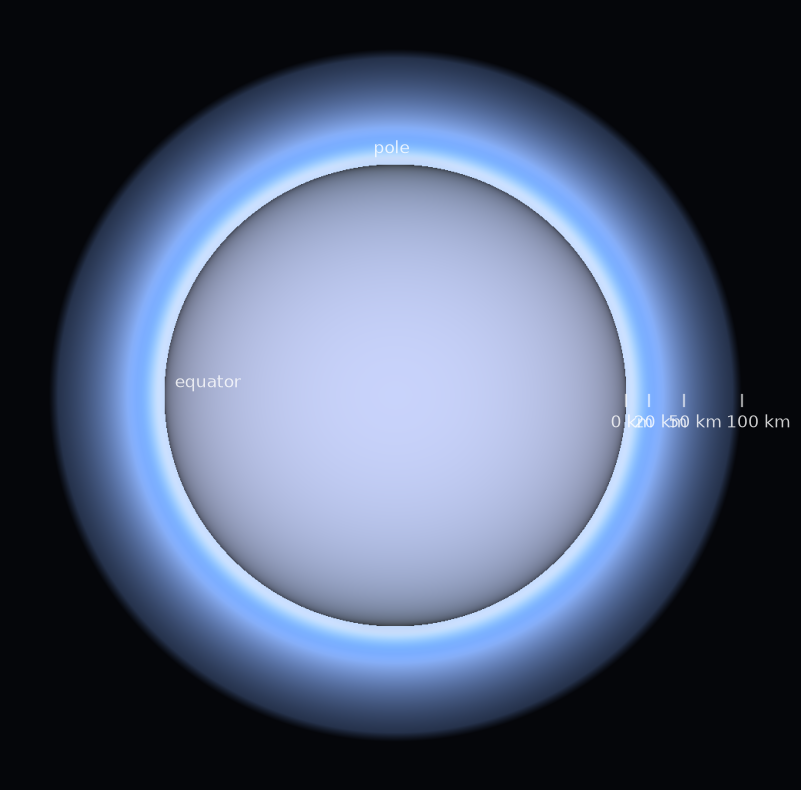
\includegraphics[width=\linewidth]{figures/globe_modern.png}\\[-1pt]{\scriptsize\sffamily\bfseries Modern}\end{minipage}\hfill
\begin{minipage}[t]{0.235\linewidth}\centering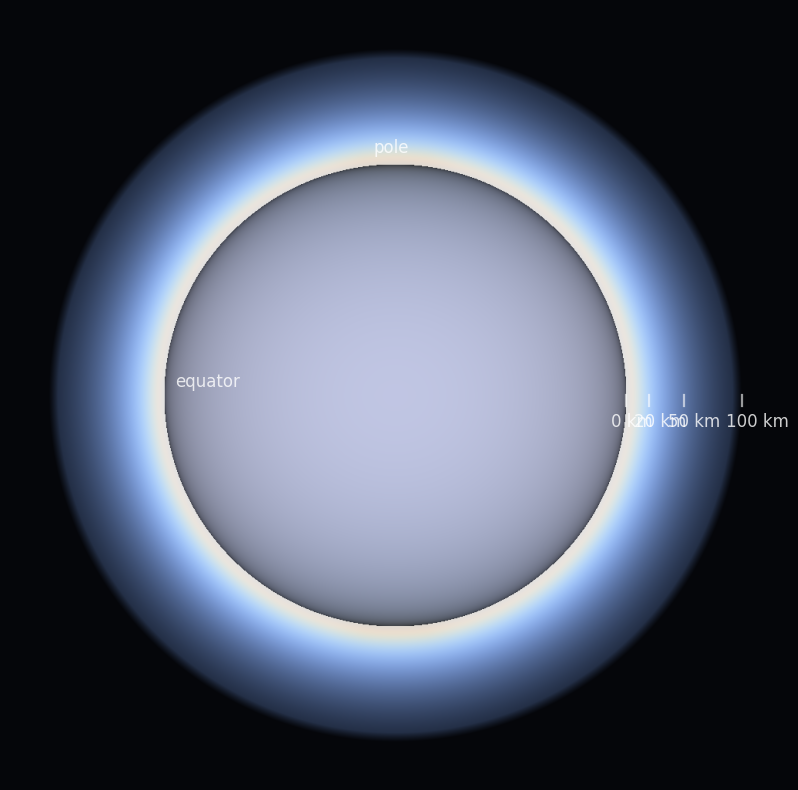
\includegraphics[width=\linewidth]{figures/globe_archean38.png}\\[-1pt]{\scriptsize\sffamily\bfseries 3.8 Ga, clear Archean}\end{minipage}\hfill
\begin{minipage}[t]{0.235\linewidth}\centering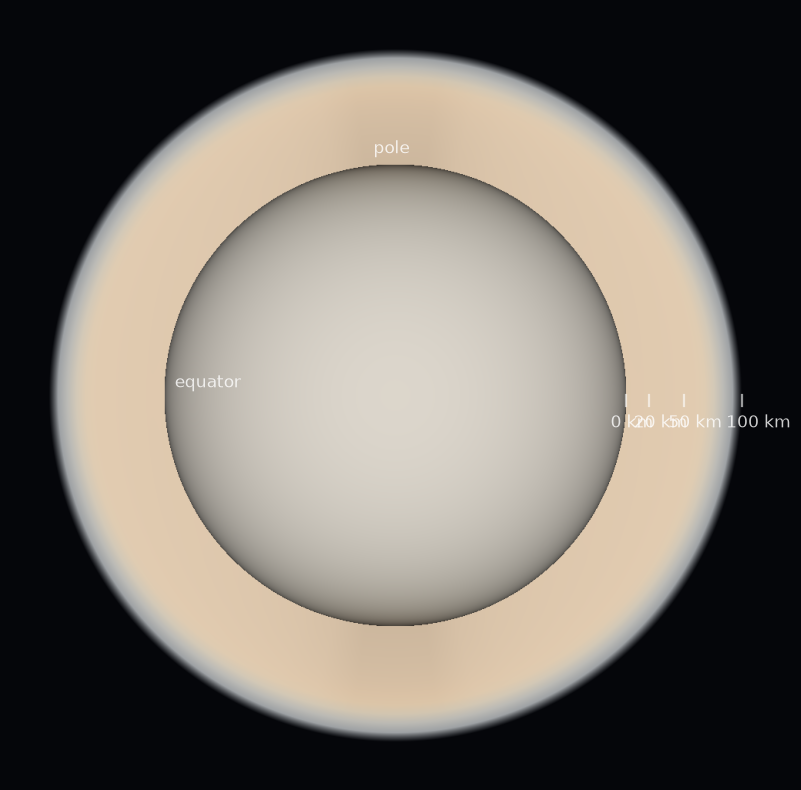
\includegraphics[width=\linewidth]{figures/globe_archean27.png}\\[-1pt]{\scriptsize\sffamily\bfseries 2.7 Ga, hazy Archean}\end{minipage}\hfill
\begin{minipage}[t]{0.235\linewidth}\centering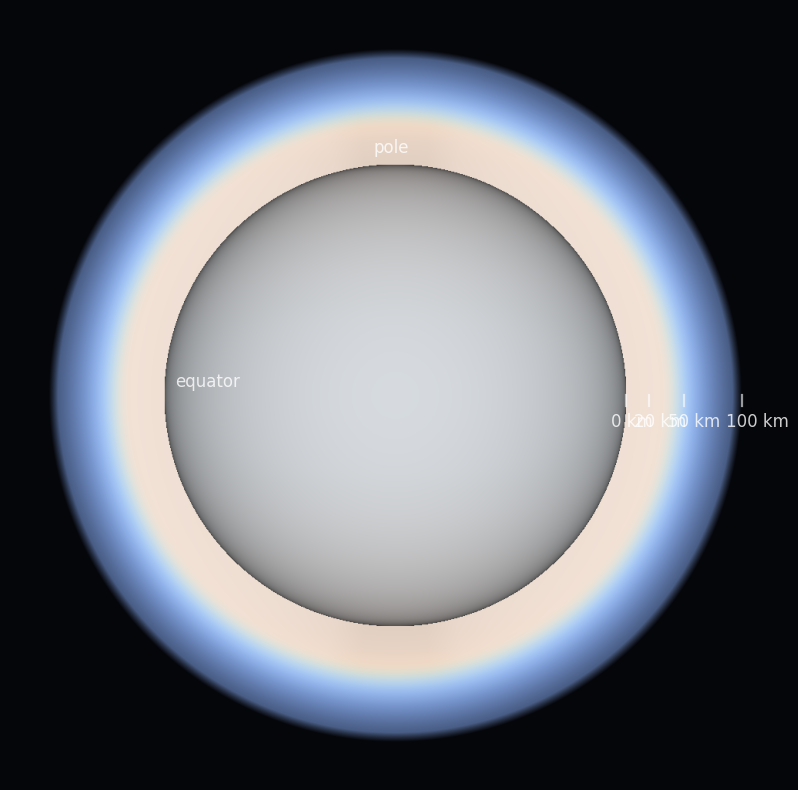
\includegraphics[width=\linewidth]{figures/globe_hadean44.png}\\[-1pt]{\scriptsize\sffamily\bfseries 4.4 Ga, 30-bar CO$_2$}\end{minipage}\\[6pt]
\begin{minipage}[t]{0.235\linewidth}\centering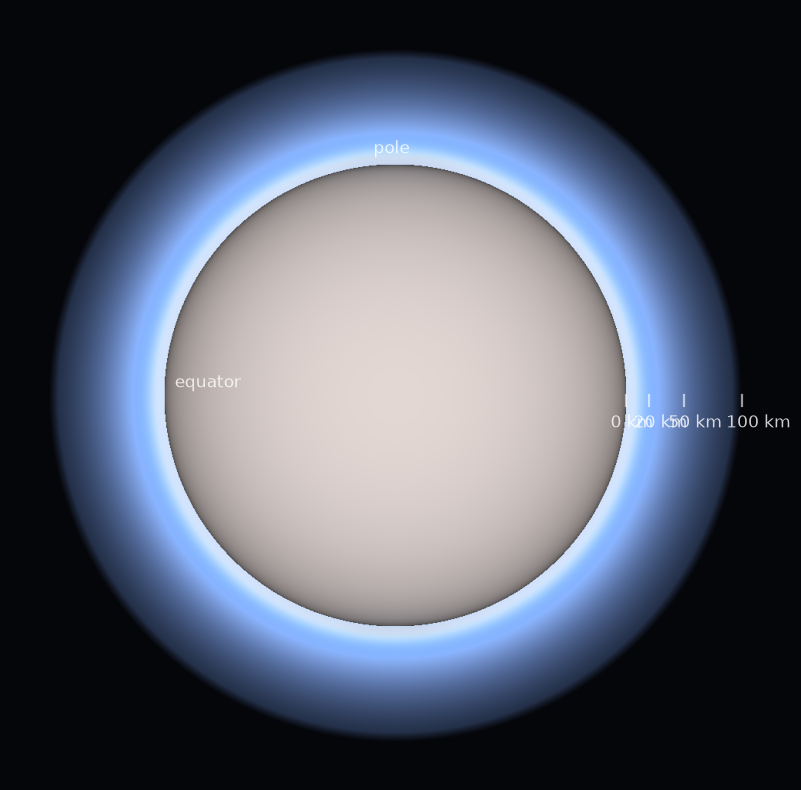
\includegraphics[width=\linewidth]{figures/globe_snowball07.png}\\[-1pt]{\scriptsize\sffamily\bfseries 700 Ma, Snowball}\end{minipage}\hfill
\begin{minipage}[t]{0.235\linewidth}\centering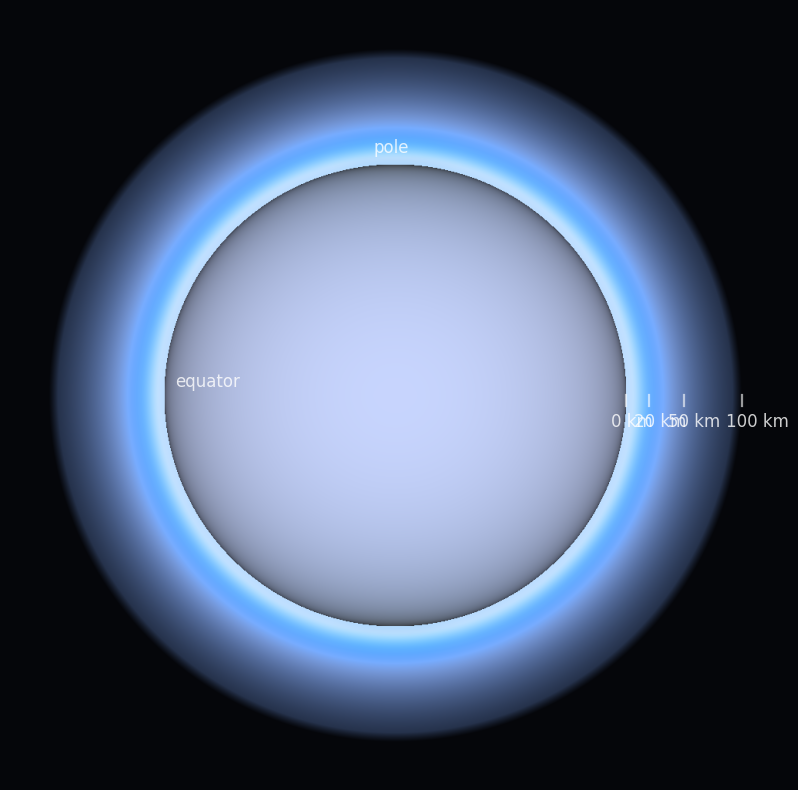
\includegraphics[width=\linewidth]{figures/globe_carbon30.png}\\[-1pt]{\scriptsize\sffamily\bfseries 300 Ma, Carboniferous}\end{minipage}\hfill
\begin{minipage}[t]{0.235\linewidth}\centering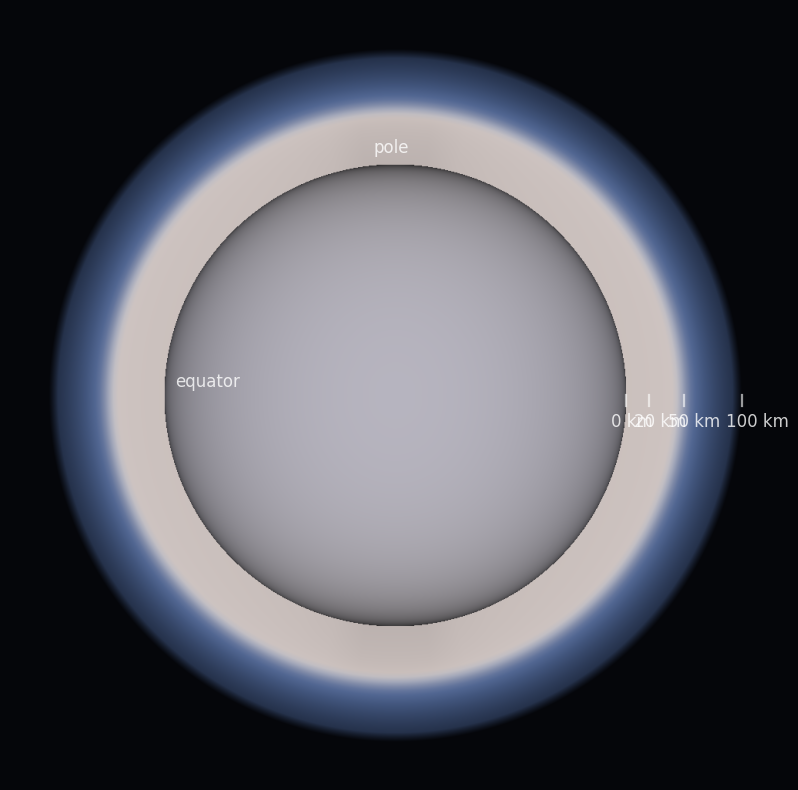
\includegraphics[width=\linewidth]{figures/globe_kpg66.png}\\[-1pt]{\scriptsize\sffamily\bfseries 66 Ma, impact winter}\end{minipage}\hfill
\begin{minipage}[t]{0.235\linewidth}\centering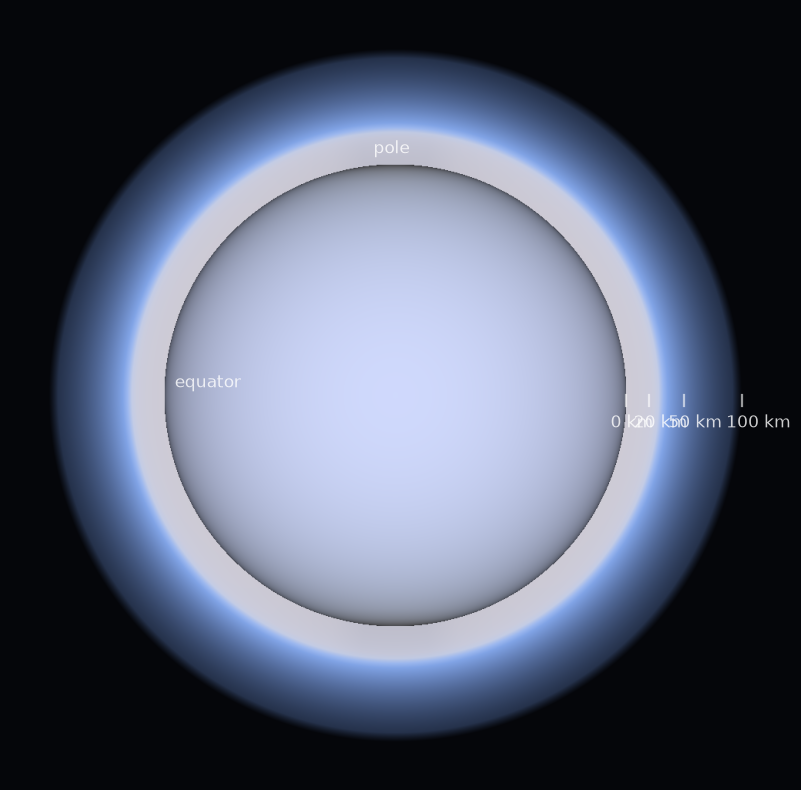
\includegraphics[width=\linewidth]{figures/globe_volcanic.png}\\[-1pt]{\scriptsize\sffamily\bfseries 1815, volcanic year}\end{minipage}\\[6pt]

\caption{Volumetric renderings of the atmosphere at eight epochs. Equinox geometry with the Sun behind the viewer; the shell is the limb color along tangent rays, drawn 30 times too thick (100\,km spans half an Earth radius); the disk is the planet's reflected color over ocean (ice for Snowball Earth). Limb brightness is compressed so faint upper layers remain visible.}
\label{fig:globes}
\end{figure*}

\footnotesize
\textbf{Modern, clean air.} Modern Earth for reference: white-blue troposphere grading to a deep blue stratosphere and fading to black, brightest at the equator and darker toward the poles.

\textbf{Early Archean, $\sim$3.8 Ga.} Clear early Archean. Structurally modern: white-blue near the surface, deep blue above, fading to black. With a little more CO$_2$ and no ozone the shell is marginally paler than today's and the disk very slightly whiter.

\textbf{Neoarchean, $\sim$2.7 Ga (thick haze).} Hazy Neoarchean. The organic haze colors the entire limb tan: every tangent ray below $\sim$60 km crosses the layer (centered $\sim$45 km) twice. Only above it does the shell turn a faint, dusty blue. The disk is the pale orange dot, though from space it is a subtle cream-orange rather than a vivid one.

\textbf{Early Hadean, $\sim$4.4 Ga.} 30-bar CO$_2$ Hadean. The shell is an opaque, luminous white-peach almost all the way up, because tangent rays at any tangent height below $\sim$60 km pass through many optical depths of CO$_2$; only the outermost fringe thins to blue. The disk is bright and nearly white: a cloudless, Rayleigh-only Venus.

\textbf{Snowball Earth, $\sim$700 Ma.} Snowball Earth. The bluest shell in the set above a blazing white disk of ice. The polar limb stays bright because the frozen surface reflects so much light back into the atmosphere.

\textbf{Carboniferous, $\sim$300 Ma.} Carboniferous, 33\% O$_2$. The extra oxygen raises total pressure by about a tenth, so the limb is marginally thicker and brighter than today's, but to the eye it is indistinguishable from modern Earth: once ozone and clean air are in place, the sky from space has been the same pale blue dot for two billion years.

\textbf{K-Pg impact winter, 66 Ma.} Impact winter. A dim brown-gray band from the soot and sulfate layer occupies the lower and middle shell; above $\sim$40 km the untouched upper atmosphere is still faintly blue. The disk is a dull gray-lilac, and dark at high latitudes.

\textbf{Volcanic year (Tambora 1815 / Toba-lite).} Volcanic year. A milky white sulfate band near 20 km sits between the white-blue troposphere and the deep blue upper shell. The disk is brighter and whiter than clean modern Earth.

\normalsize

\Needspace*{20\baselineskip}
\section*{Epoch by epoch}
The eighteen panels that follow are laid out identically so they can be compared at a glance. Each panel begins with the epoch's name and a one-line summary of the atmosphere assumed (Table~\ref{tab:epochs} gives the full parameters). The upper row shows the noon sky dome at three latitudes---the equator, a mid-latitude site and the summer pole---with the zenith at the top of each swatch and the horizon at the bottom, the correlated color temperatures of both printed above, and the Sun's disk drawn in its own color, at its noon elevation, and with a brightness that reflects how much of it survives the atmosphere (where the Sun would not be visible at all, the swatch says so). The two strips beneath trace the sky from the solar horizon across the zenith to the antisolar horizon at two moments: with the Sun sitting on the horizon, and with it $4^\circ$ below, in civil twilight. All swatches are shown at a brightness relative to today's clean sky, so a dim epoch reads as dim; the paragraph after each panel explains what the colors mean and why they arise.

\par\vspace{6pt}\noindent\begin{minipage}{\linewidth}
{\normalsize\bfseries Early Hadean, $\sim$4.4 Ga\par}
{\small\itshape post-magma-ocean CO$_2$/steam atmosphere ($\sim$30 bar CO$_2$)\par}\vspace{3pt}
\centering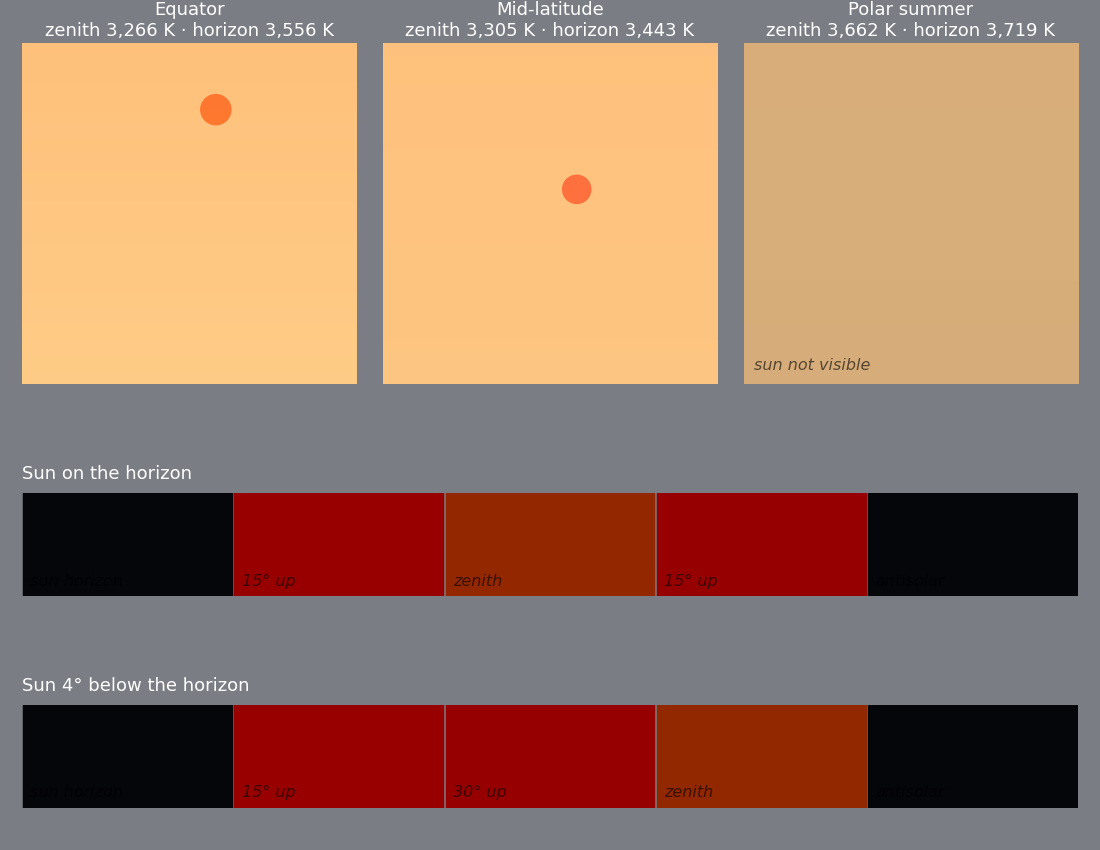
\includegraphics[width=\linewidth]{figures/sky_hadean44.png}
\captionof{figure}{Early Hadean, $\sim$4.4 Ga. Top: noon sky dome at the equator, mid-latitude and polar summer, zenith at top, horizon at bottom, Sun's disk in its own color. Below: sky from the solar horizon to the antisolar horizon with the Sun on the horizon and $4^\circ$ below it.}
\end{minipage}\par\vspace{4pt}
A $\sim$30-bar CO$_2$ atmosphere has a Rayleigh optical depth near 5 at 550 nm and about 18 in the violet, so blue light is scattered back to space many times before it reaches the ground. What arrives is a diffuse, shadowless, peach-white glow of $\sim$3,300 K, nearly identical from zenith to horizon, under a young Sun that is only 70\% as bright. The Sun itself is a dim ember at the equator and vanishes entirely at mid and high latitudes: this is a Venus-like sky. Sunset is a brief, deep-orange dimming of the whole dome rather than an event at the horizon.

\par\vspace{6pt}\noindent\begin{minipage}{\linewidth}
{\normalsize\bfseries Late Hadean, $\sim$4.0 Ga\par}
{\small\itshape CO$_2$ mostly drawn down into carbonate; $\sim$1 bar N$_2$, $\sim$0.5 bar CO$_2$\par}\vspace{3pt}
\centering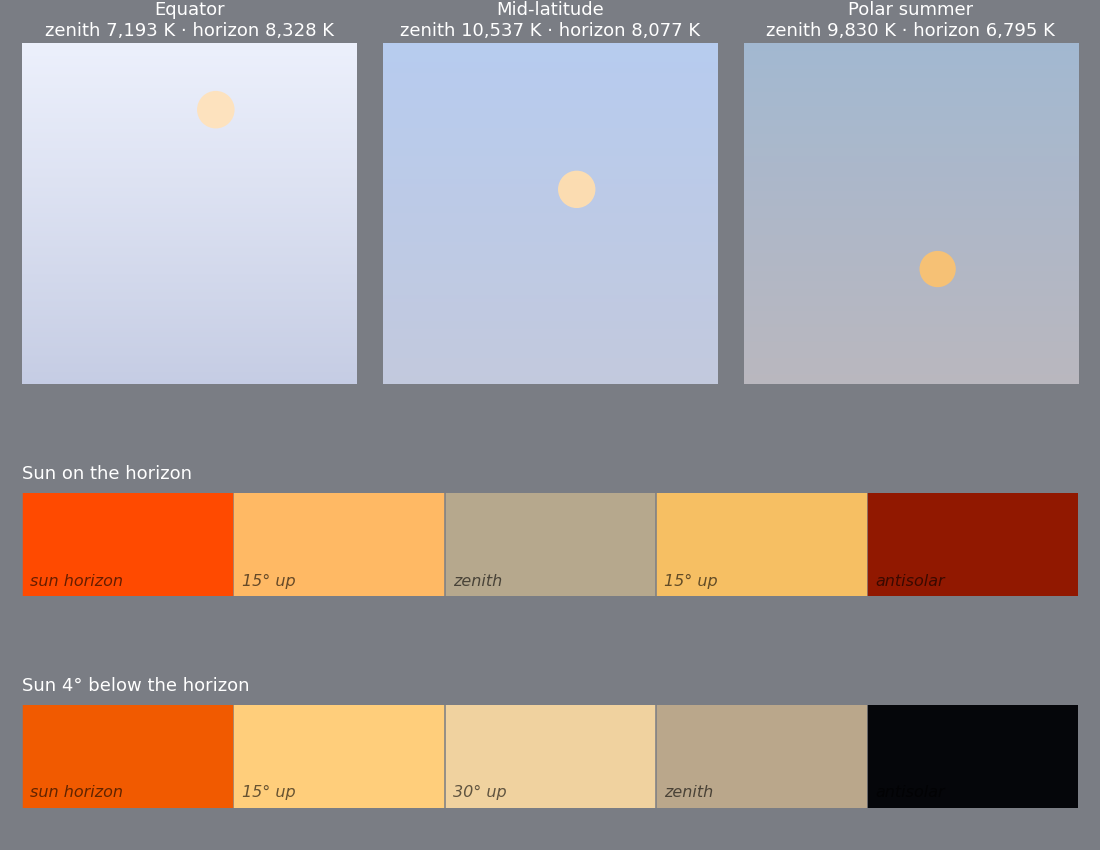
\includegraphics[width=\linewidth]{figures/sky_hadean40.png}
\captionof{figure}{Late Hadean, $\sim$4.0 Ga. Top: noon sky dome at the equator, mid-latitude and polar summer, zenith at top, horizon at bottom, Sun's disk in its own color. Below: sky from the solar horizon to the antisolar horizon with the Sun on the horizon and $4^\circ$ below it.}
\end{minipage}\par\vspace{4pt}
Once most of the CO$_2$ has gone into carbonate, Rayleigh scattering falls to roughly twice the modern value. The sky turns pale blue at the zenith but conspicuously whiter than today (7,000--10,500 K versus 9,000--15,000 K), because the extra scattering fills the dome with multiply-scattered white light. Horizons are milky. The setting Sun is deep red and the twilight zenith, with no ozone yet, is cream rather than blue.

\par\vspace{6pt}\noindent\begin{minipage}{\linewidth}
{\normalsize\bfseries Early Archean, $\sim$3.8 Ga\par}
{\small\itshape haze-free, anoxic; CO$_2$ $\sim$0.1 bar, CH$_4$ $\sim$1000 ppm, no ozone\par}\vspace{3pt}
\centering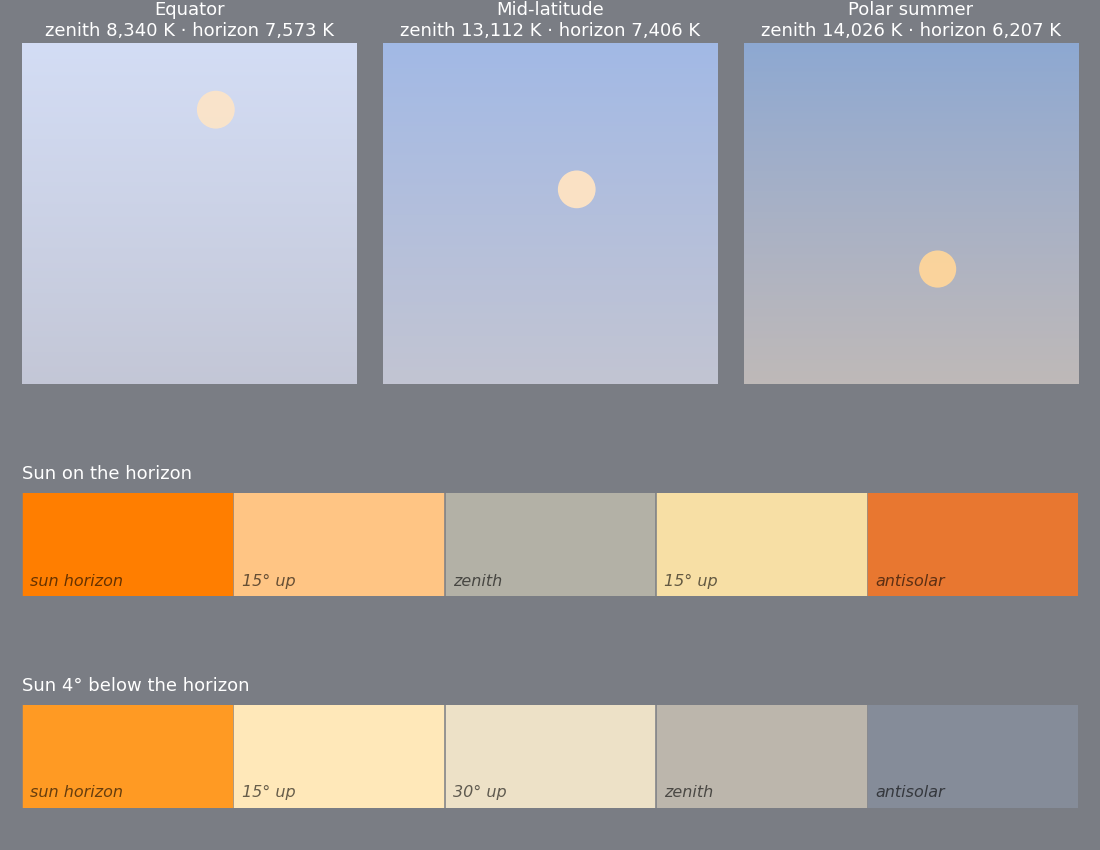
\includegraphics[width=\linewidth]{figures/sky_archean38.png}
\captionof{figure}{Early Archean, $\sim$3.8 Ga. Top: noon sky dome at the equator, mid-latitude and polar summer, zenith at top, horizon at bottom, Sun's disk in its own color. Below: sky from the solar horizon to the antisolar horizon with the Sun on the horizon and $4^\circ$ below it.}
\end{minipage}\par\vspace{4pt}
With CO$_2$ down to $\sim$0.1 bar, noon skies are close to modern blue, only slightly whiter. The unmistakable difference is at dusk. The blue of the modern twilight zenith is produced by ozone absorbing yellow-orange light (the Chappuis band) along the long grazing path; with no free O$_2$ there is no ozone, so the Archean twilight zenith is a pale yellow-cream, and the whole sky fades from blue to beige to orange as the Sun sets. Sunsets themselves are much like today's, slightly redder from the extra CO$_2$ and dimmer Sun.

\par\vspace{6pt}\noindent\begin{minipage}{\linewidth}
{\normalsize\bfseries Neoarchean, $\sim$2.7 Ga (thin haze)\par}
{\small\itshape biogenic CH$_4$/CO$_2$ $\sim$0.1: intermittent thin organic haze\par}\vspace{3pt}
\centering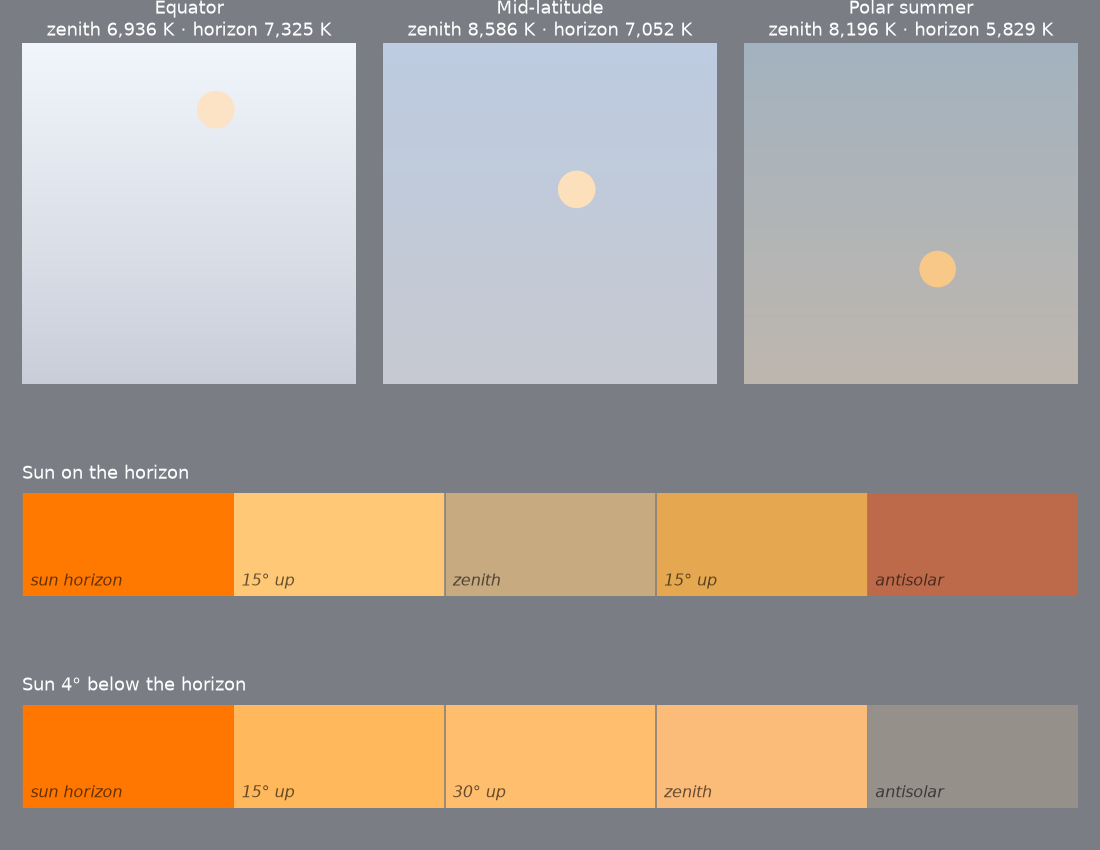
\includegraphics[width=\linewidth]{figures/sky_archean27thin.png}
\captionof{figure}{Neoarchean, $\sim$2.7 Ga (thin haze). Top: noon sky dome at the equator, mid-latitude and polar summer, zenith at top, horizon at bottom, Sun's disk in its own color. Below: sky from the solar horizon to the antisolar horizon with the Sun on the horizon and $4^\circ$ below it.}
\end{minipage}\par\vspace{4pt}
An intermittent organic haze at optical depth $\sim$0.15 pushes the zenith toward a pastel, milk-blue (7,000--8,500 K) and lays a warm cast on the horizon; at the poles, where sunlight crosses the haze obliquely, the horizon turns visibly cream. Twilight is orange all the way to the zenith.

\par\vspace{6pt}\noindent\begin{minipage}{\linewidth}
{\normalsize\bfseries Neoarchean, $\sim$2.7 Ga (thick haze)\par}
{\small\itshape "Pale Orange Dot": Titan-like fractal organic haze, $\tau_{550}$$\sim$0.6\par}\vspace{3pt}
\centering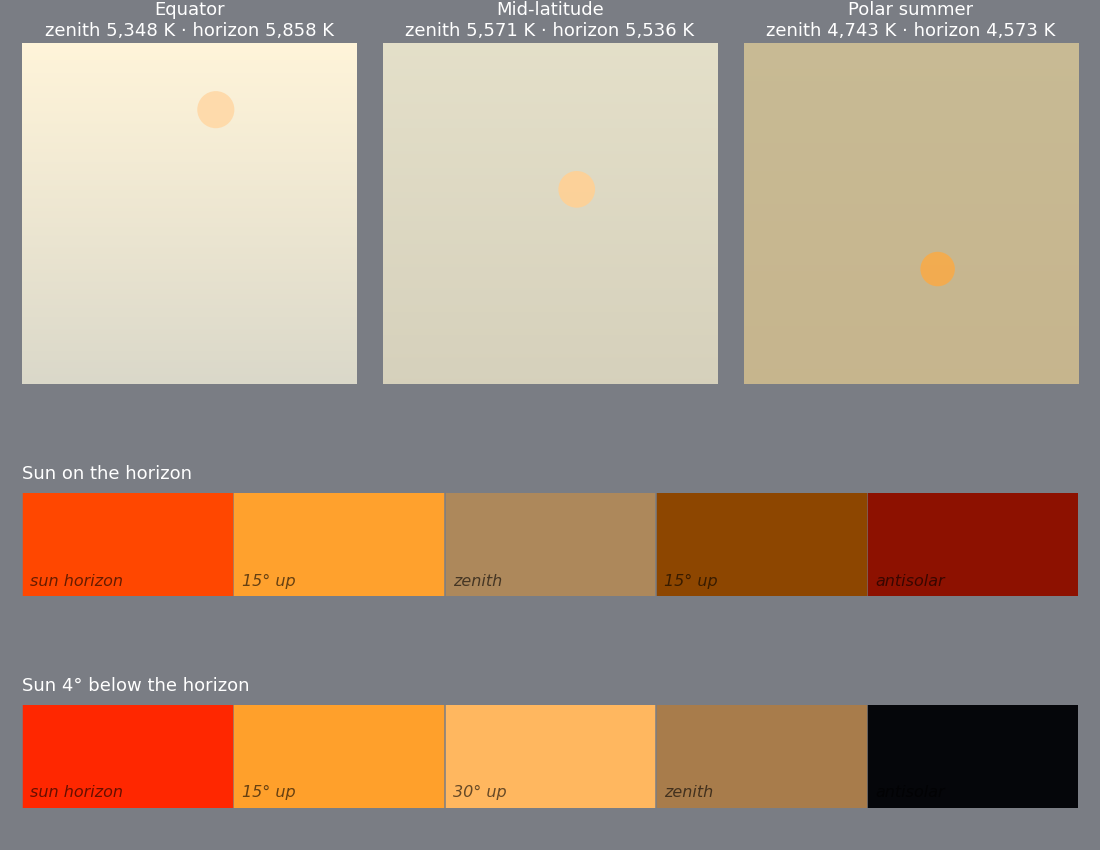
\includegraphics[width=\linewidth]{figures/sky_archean27.png}
\captionof{figure}{Neoarchean, $\sim$2.7 Ga (thick haze). Top: noon sky dome at the equator, mid-latitude and polar summer, zenith at top, horizon at bottom, Sun's disk in its own color. Below: sky from the solar horizon to the antisolar horizon with the Sun on the horizon and $4^\circ$ below it.}
\end{minipage}\par\vspace{4pt}
This is the 'Pale Orange Dot' seen from below. At optical depth $\sim$0.6 the haze absorbs blue and scatters forward, so the entire dome is a warm cream to pale tan ($\sim$5,300 K at the equator, $\sim$4,700 K at the poles) with almost no zenith-to-horizon gradient: the sky looks like a bright overcast made of orange-tinted glass. The Sun is a soft, defined disk (haze scatters strongly forward) at 4,100 K. Sunsets are deep and long: the solar horizon reaches vermilion, the sky 15$^\circ$ above the Sun is amber, and the antisolar sky is peach rather than pink.

\par\vspace{6pt}\noindent\begin{minipage}{\linewidth}
{\normalsize\bfseries Neoarchean, $\sim$2.7 Ga (very thick haze)\par}
{\small\itshape upper-end haze, $\tau_{550}$$\sim$1.5: CH$_4$/CO$_2$ well above 0.2\par}\vspace{3pt}
\centering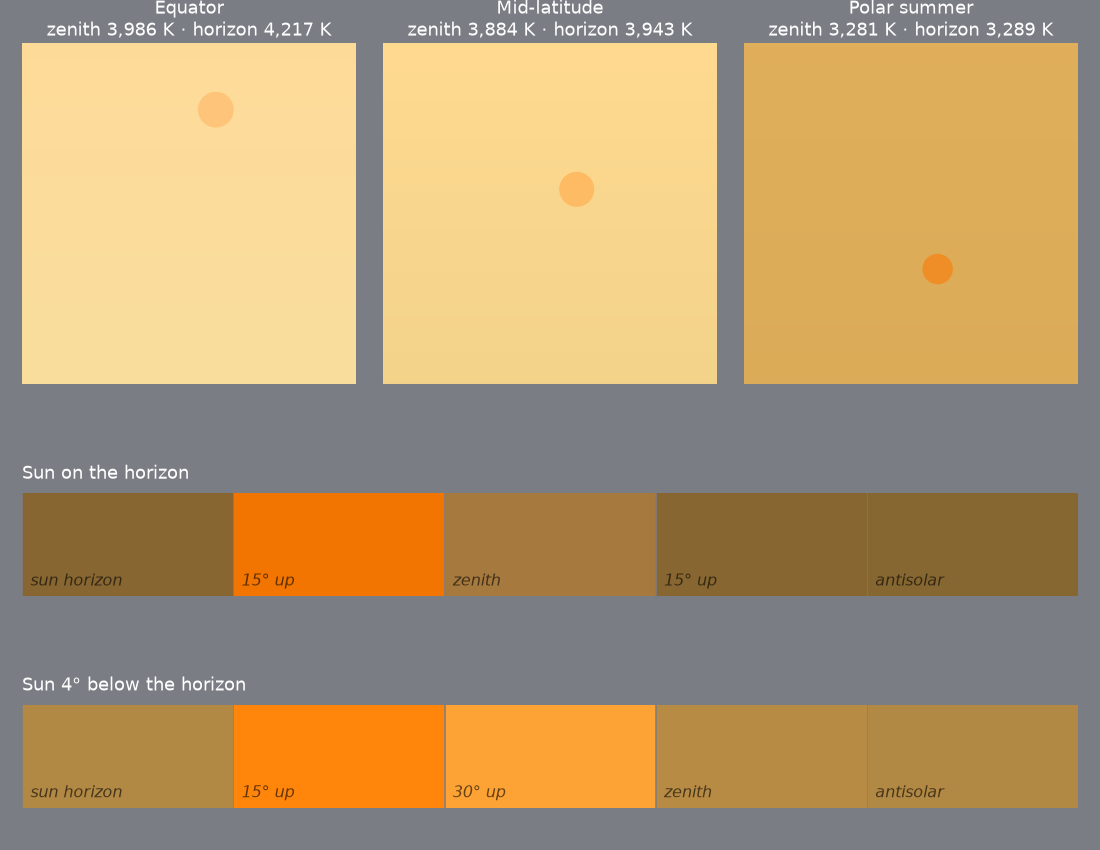
\includegraphics[width=\linewidth]{figures/sky_archean27vthick.png}
\captionof{figure}{Neoarchean, $\sim$2.7 Ga (very thick haze). Top: noon sky dome at the equator, mid-latitude and polar summer, zenith at top, horizon at bottom, Sun's disk in its own color. Below: sky from the solar horizon to the antisolar horizon with the Sun on the horizon and $4^\circ$ below it.}
\end{minipage}\par\vspace{4pt}
At the upper end of plausible haze ($\tau\approx$1.5) the sky is a uniform saturated apricot (3,300--4,200 K), fully Titan-like, and the polar Sun is reduced to an orange smear. Anything below this haze would have had roughly 20--30\% of the surface sunlight of a clear sky.

\par\vspace{6pt}\noindent\begin{minipage}{\linewidth}
{\normalsize\bfseries Paleoproterozoic, $\sim$2.2 Ga\par}
{\small\itshape after the Great Oxidation Event: O$_2$ $\sim$1\% PAL, ozone column 66 DU\par}\vspace{3pt}
\centering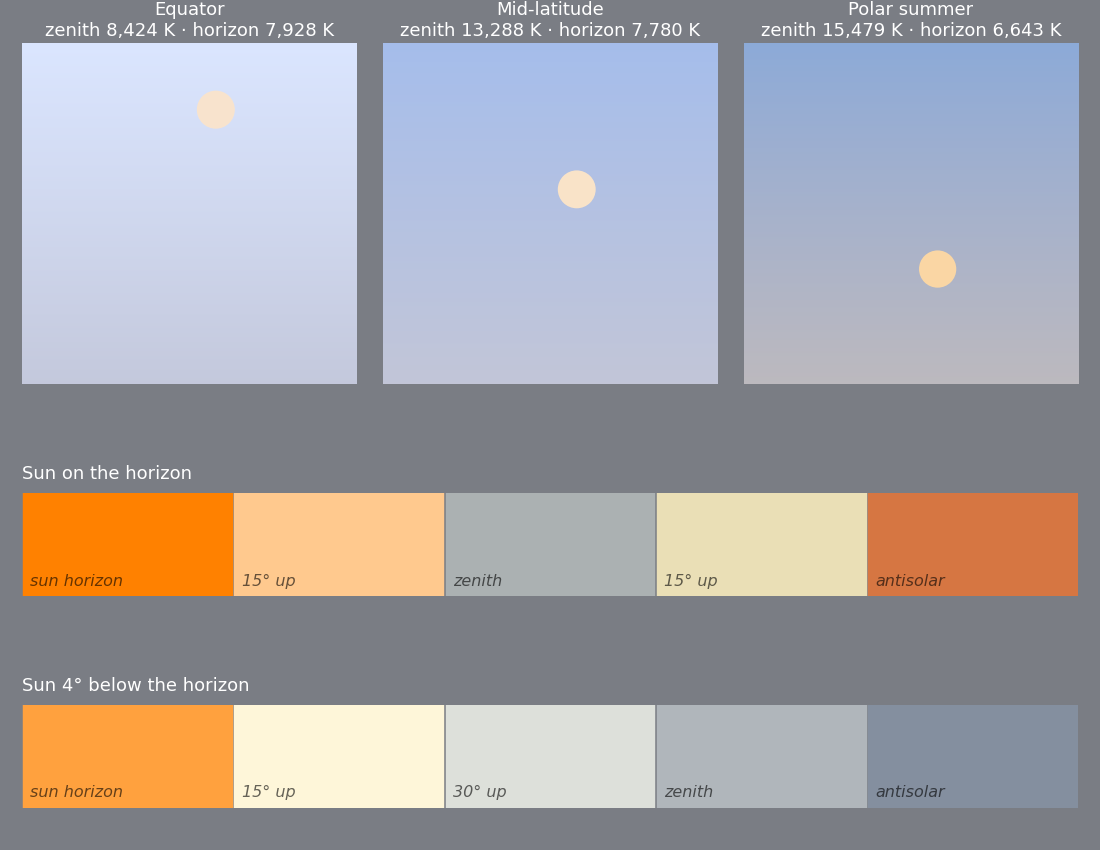
\includegraphics[width=\linewidth]{figures/sky_proterozoic22.png}
\captionof{figure}{Paleoproterozoic, $\sim$2.2 Ga. Top: noon sky dome at the equator, mid-latitude and polar summer, zenith at top, horizon at bottom, Sun's disk in its own color. Below: sky from the solar horizon to the antisolar horizon with the Sun on the horizon and $4^\circ$ below it.}
\end{minipage}\par\vspace{4pt}
After the Great Oxidation Event, about 1\% of today's O$_2$ builds an ozone column of 66 DU, the Cooke et al. (2021) global mean for that oxygen level: about a fifth of a modern mid-latitude column, not the half that older estimates gave. Noon skies are already modern blue. Twilight is where the thin column shows. With the Sun 4$^\circ$ below the horizon the zenith leaves the cream of an ozone-free dusk ($\sim$6,000 K) and becomes a pale blue-gray ($\sim$7,100 K). It is not yet the deep blue of a 300 DU twilight ($\sim$12,500 K). That saturated blue dusk is in place once the column is near modern, as in the snowball sky at 169 DU. (The pink antisolar arch needs no ozone: it is a Rayleigh effect and shows up faintly even in the Hadean model.)

\par\vspace{6pt}\noindent\begin{minipage}{\linewidth}
{\normalsize\bfseries Snowball Earth, $\sim$700 Ma\par}
{\small\itshape cold, dry, very clean air; ice/snow surface (albedo 0.75); ozone 169 DU\par}\vspace{3pt}
\centering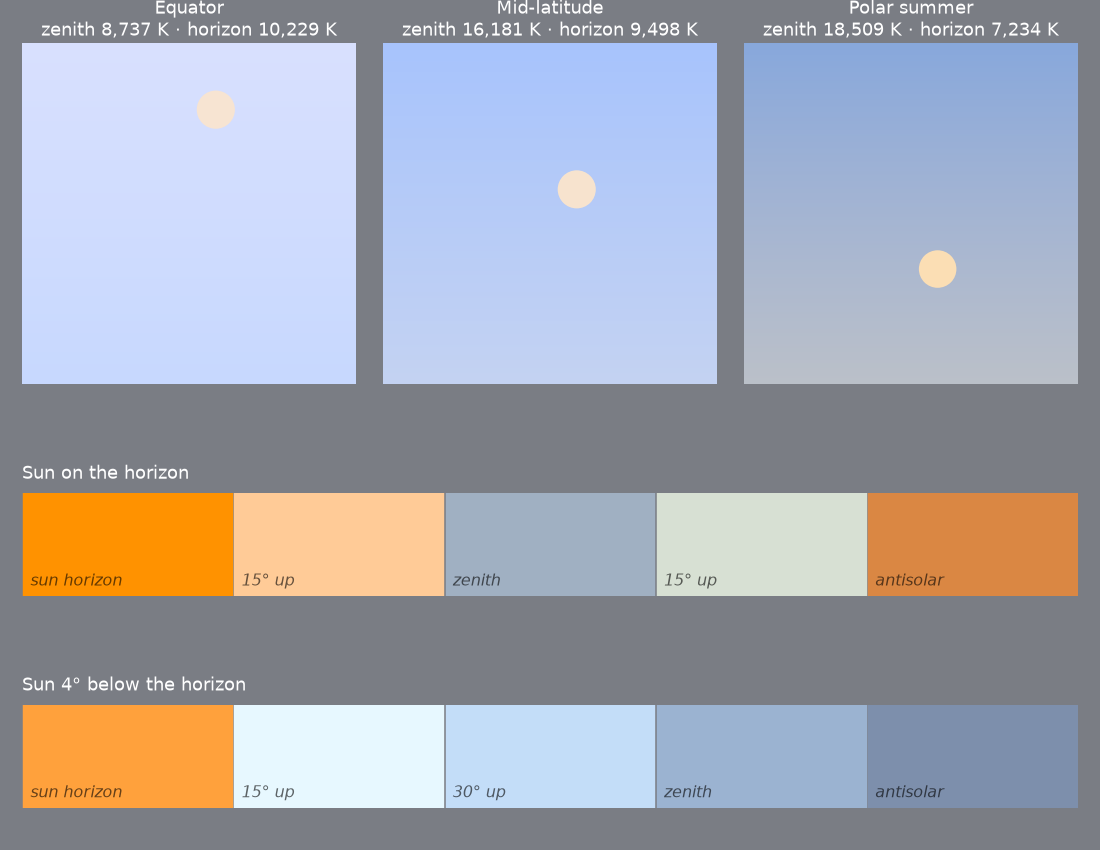
\includegraphics[width=\linewidth]{figures/sky_snowball07.png}
\captionof{figure}{Snowball Earth, $\sim$700 Ma. Top: noon sky dome at the equator, mid-latitude and polar summer, zenith at top, horizon at bottom, Sun's disk in its own color. Below: sky from the solar horizon to the antisolar horizon with the Sun on the horizon and $4^\circ$ below it.}
\end{minipage}\par\vspace{4pt}
A frozen planet has a dry, exceptionally clean atmosphere and a surface albedo near 0.75. The result is the bluest sky in Earth's history: 9,000 K at the equatorial zenith and over 20,000 K over polar ice, with horizons that stay distinctly blue instead of whitening, because the sunlit ice floods the sky from below with blue-white light. Sunsets are golden and comparatively pale; there is little aerosol to redden them.

\par\vspace{6pt}\noindent\begin{minipage}{\linewidth}
{\normalsize\bfseries Ordovician meteor storm, $\sim$466 Ma\par}
{\small\itshape after the L-chondrite parent body broke up: O$_2$ $\sim$17\%, CO$_2$ $\sim$2,500 ppm, a little meteoric dust aloft\par}\vspace{3pt}
\centering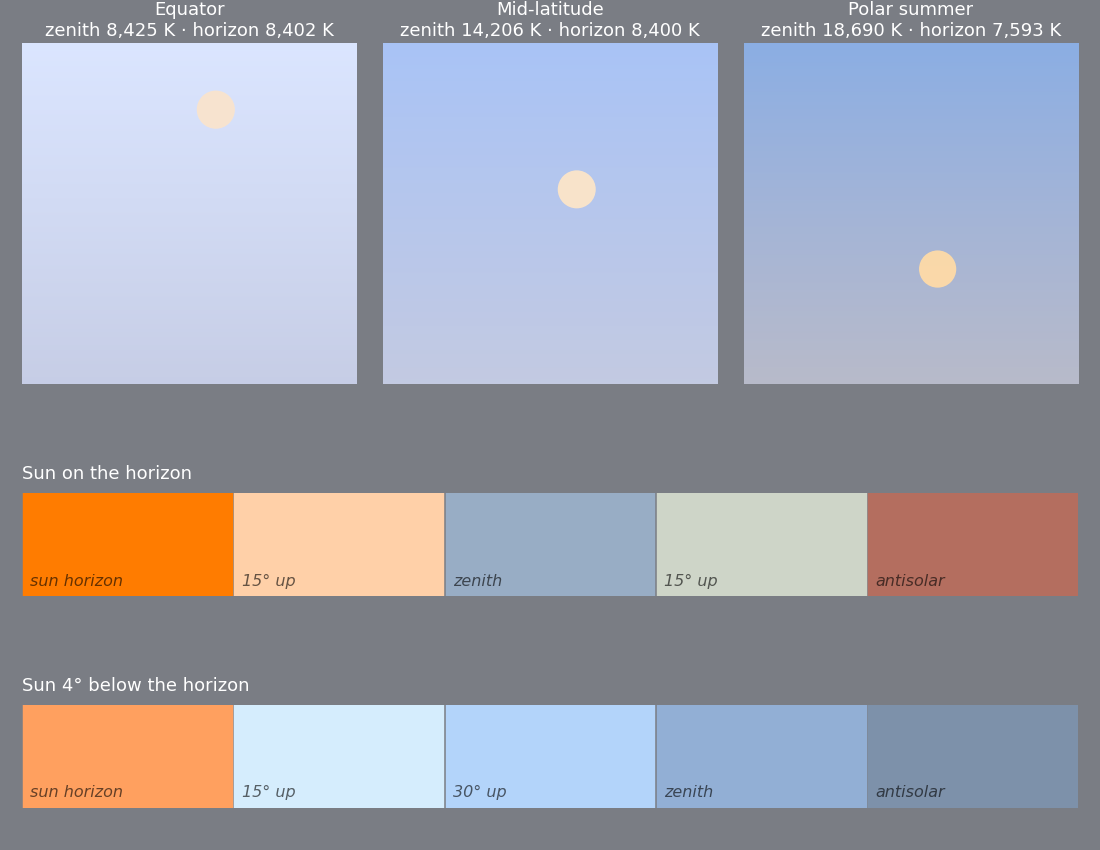
\includegraphics[width=\linewidth]{figures/sky_ordovician466.png}
\captionof{figure}{Ordovician meteor storm, $\sim$466 Ma. Top: noon sky dome at the equator, mid-latitude and polar summer, zenith at top, horizon at bottom, Sun's disk in its own color. Below: sky from the solar horizon to the antisolar horizon with the Sun on the horizon and $4^\circ$ below it.}
\end{minipage}\par\vspace{4pt}
About 466 million years ago the L-chondrite parent body, an asteroid about 150 km across, was shattered in the main belt, and its fragments still make up almost a third of the meteorites that fall today. For more than two million years the fine dust reaching Earth rose a thousandfold or more, and decimetre stones about a hundredfold: fossil meteorites lie scattered through Swedish limestones of that age, and the dust may have helped tip the climate toward the Late Ordovician ice age (Schmitz et al. 2019). The meteors here come a hundred times as often as today, most of them slow and yellow with sodium, and the zodiacal light is taken as thirty times today's, a glowing band along the ecliptic. The ring is speculation: all 21 known Ordovician craters lie within 30$^\circ$ of the palaeo-equator, which led Tomkins, Martin \& Cawood (2024) to propose that a large fragment broke up inside the Roche limit into a ring that lasted tens of millions of years; it is drawn as a faint, sunlit band that Earth's shadow cuts at night, with its debris falling at the equator as slow fireballs from the west. The air itself is close to today's: about 17\% oxygen, 2,500 ppm CO$_2$, an ozone layer within a few percent of the modern one, under a Sun 4\% fainter, so the day sky is today's blue.

\par\vspace{6pt}\noindent\begin{minipage}{\linewidth}
{\normalsize\bfseries Carboniferous, $\sim$300 Ma\par}
{\small\itshape O$_2$ $\sim$30-35\%; total pressure $\sim$1.1 bar; wildfire smoke common\par}\vspace{3pt}
\centering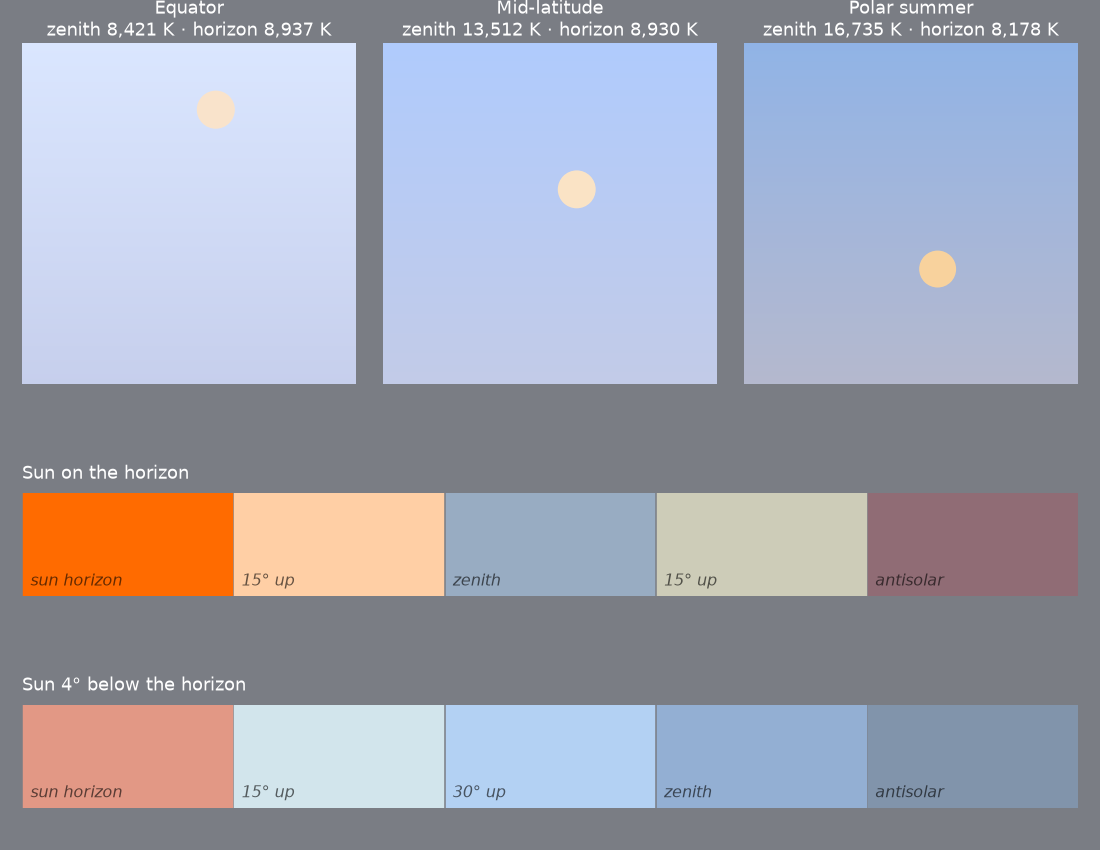
\includegraphics[width=\linewidth]{figures/sky_carbon30.png}
\captionof{figure}{Carboniferous, $\sim$300 Ma. Top: noon sky dome at the equator, mid-latitude and polar summer, zenith at top, horizon at bottom, Sun's disk in its own color. Below: sky from the solar horizon to the antisolar horizon with the Sun on the horizon and $4^\circ$ below it.}
\end{minipage}\par\vspace{4pt}
Thirty-plus percent O$_2$ raises the total pressure and Rayleigh scattering by $\sim$10\%, so skies are marginally brighter and horizons a touch whiter than today; the effect is subtle. Frequent wildfire smoke in the high-O$_2$ world would have produced red suns and brown-orange horizons far more often than in the modern era.

\par\vspace{6pt}\noindent\begin{minipage}{\linewidth}
{\normalsize\bfseries K-Pg impact winter, 66 Ma\par}
{\small\itshape months after Chicxulub: stratospheric soot (tau$\sim$1.5) + sulfate (tau$\sim$0.5)\par}\vspace{3pt}
\centering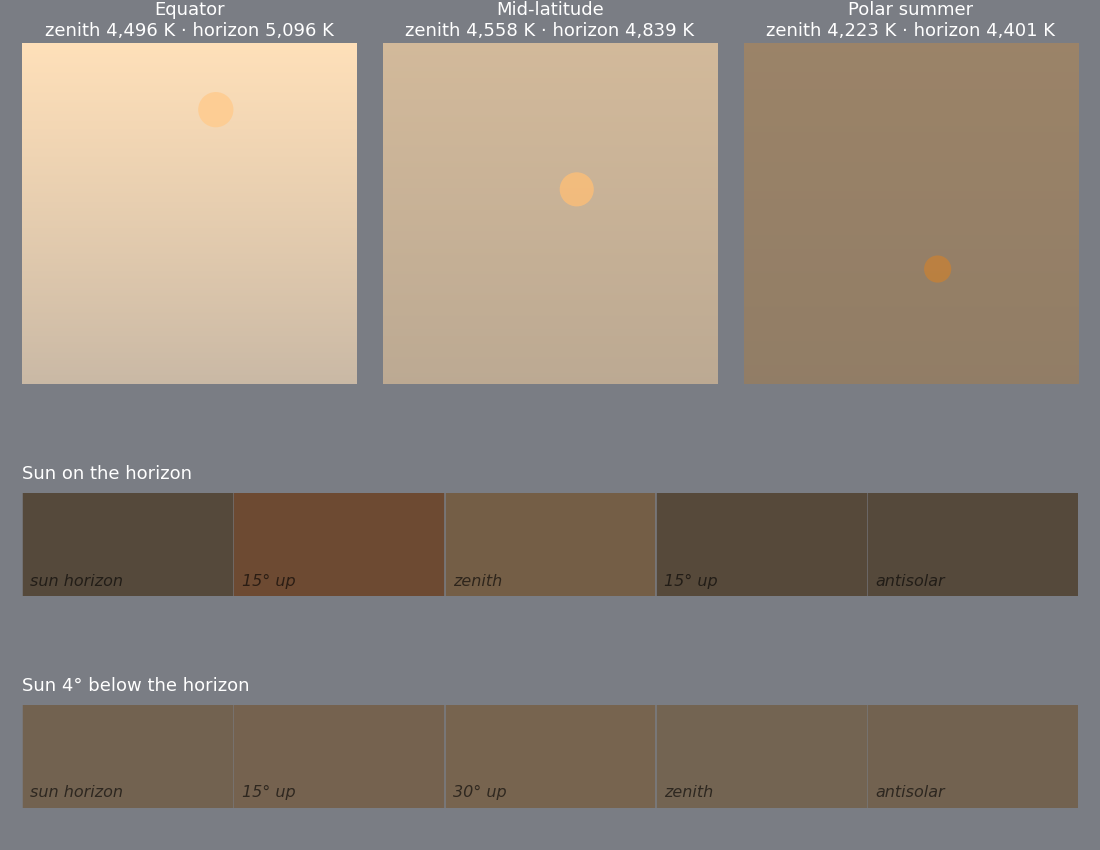
\includegraphics[width=\linewidth]{figures/sky_kpg66.png}
\captionof{figure}{K-Pg impact winter, 66 Ma. Top: noon sky dome at the equator, mid-latitude and polar summer, zenith at top, horizon at bottom, Sun's disk in its own color. Below: sky from the solar horizon to the antisolar horizon with the Sun on the horizon and $4^\circ$ below it.}
\end{minipage}\par\vspace{4pt}
Months after the Chicxulub impact, a global stratospheric layer of soot and sulfate turns the sky into a dim, uniform amber-beige (4,200--5,100 K) with no blue at all, about one-fifth as bright as a clear sky at the equator and 20$\times$ dimmer at high latitudes. The Sun is a pale orange disk at low latitudes and effectively gone near the poles. Sunsets do not happen as color events: the whole dome simply fades to dark brown, and the twilight sky is gray.

\par\vspace{6pt}\noindent\begin{minipage}{\linewidth}
{\normalsize\bfseries $\zeta$ Ophiuchi supernova, $\sim$1.78 Ma\par}
{\small\itshape clean Early Pleistocene air, under a magnitude $-$11.6 supernova in Scorpius\par}\vspace{3pt}
\centering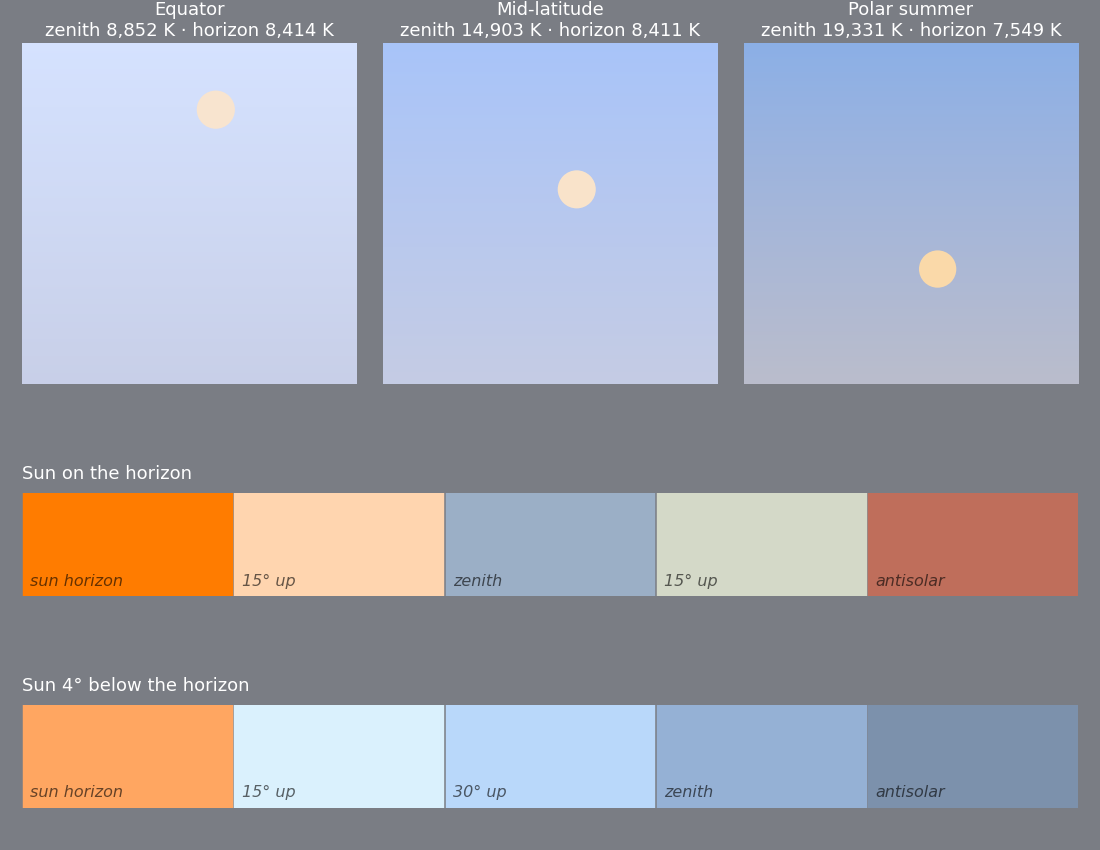
\includegraphics[width=\linewidth]{figures/sky_modern.png}
\captionof{figure}{$\zeta$ Ophiuchi supernova, $\sim$1.78 Ma. Top: noon sky dome at the equator, mid-latitude and polar summer, zenith at top, horizon at bottom, Sun's disk in its own color. Below: sky from the solar horizon to the antisolar horizon with the Sun on the horizon and $4^\circ$ below it.}
\end{minipage}\par\vspace{4pt}
About 1.78 million years ago a star of 16 to 18 solar masses exploded in a binary in the Scorpius-Centaurus association. The explosion unbound its companion, which is now the runaway O star $\zeta$ Ophiuchi, and left a neutron star that is now the pulsar PSR B1706-16; tracing both back puts the explosion 1.78 $\pm$ 0.21 Myr ago at 107 $\pm$ 4 pc (Neuhäuser et al. 2019). Its iron-60 may be part of the 1.5 to 3.2 Myr old $^{60}$Fe found in deep-sea crusts and on the Moon. A typical Type II-P supernova (Richardson et al. 2014) at that distance peaks near $-$11.6, about twice as bright as Geminga's, or $-$12.3 if the binary stripped the star and made it a Type Ib. The paper's abstract gives no sky position, so the star is drawn where a straight-line trace of $\zeta$ Oph's present motion puts it, near RA 16h10m, Dec $-$21$^\circ$. The stars are moved back along their measured space motions too; Antares has since travelled about 12$^\circ$, and in the sky of the time the supernova sat about 12$^\circ$ west of it. That trace lands at 130 to 140 pc rather than 107, so the position is approximate. From mid-northern latitudes it stays low in the south. The air is clean Early Pleistocene air.

\par\vspace{6pt}\noindent\begin{minipage}{\linewidth}
{\normalsize\bfseries Geminga supernova, $\sim$342 ka\par}
{\small\itshape clean Middle Pleistocene air, under a magnitude $-$11 supernova in Orion\par}\vspace{3pt}
\centering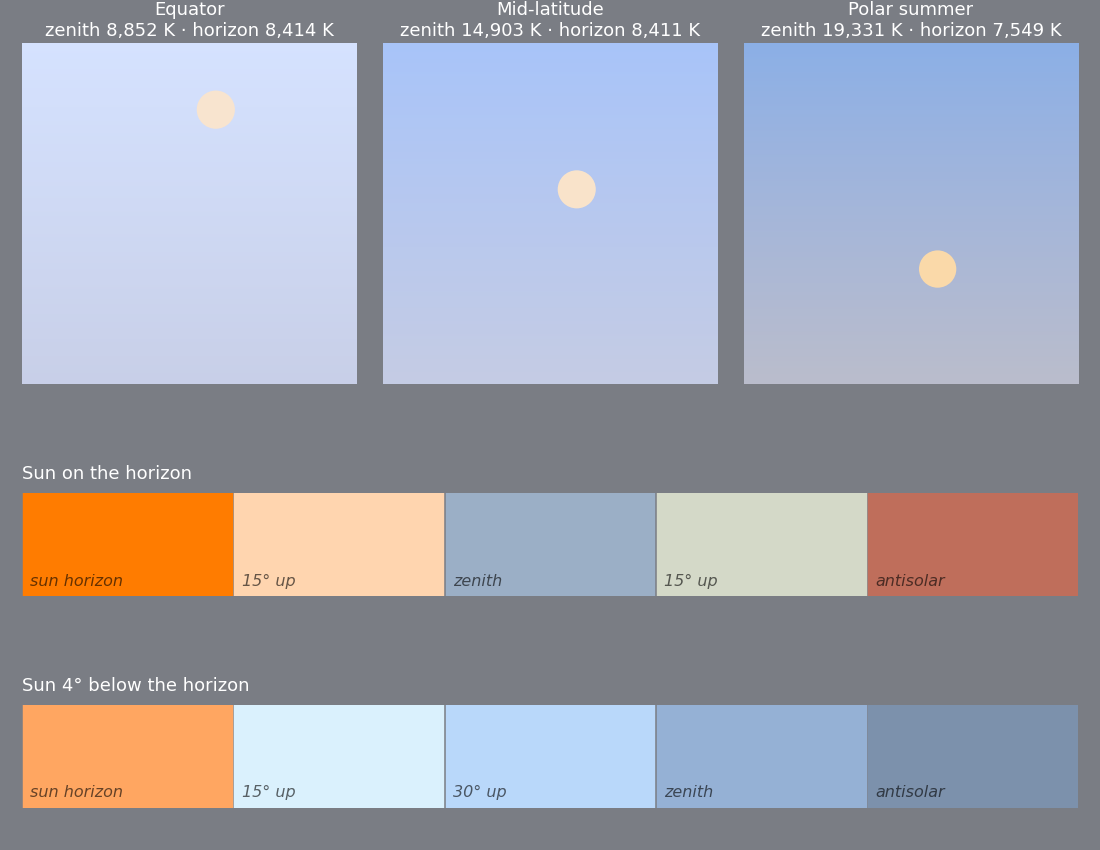
\includegraphics[width=\linewidth]{figures/sky_modern.png}
\captionof{figure}{Geminga supernova, $\sim$342 ka. Top: noon sky dome at the equator, mid-latitude and polar summer, zenith at top, horizon at bottom, Sun's disk in its own color. Below: sky from the solar horizon to the antisolar horizon with the Sun on the horizon and $4^\circ$ below it.}
\end{minipage}\par\vspace{4pt}
About 342,000 years ago, going by the spin-down age of the pulsar it left behind (Salvati and Sacco 2008), a star of at most 15 solar masses exploded 90 to 240 pc away, in the direction of Orion (Pellizza et al. 2005). Type II-P supernovae peak near absolute magnitude $-$16.75 (Richardson et al. 2014), so from the middle of that range, 147 pc, it reached about $-$11: a fifth of the full Moon's light, all from a point. The $-$13 often quoted needs both the near end of the distance range and an unusually bright explosion. It burned in the daytime sky as a dazzling star, cast sharp shadows at night, and held near peak for the three months of its plateau. The air is clean Middle Pleistocene air; at this distance the explosion barely touches the atmosphere (Thomas et al. 2016), so the sky's colors are today's. The star is drawn at the birthplace. The stars around it are moved back along their measured space motions, which puts it just 1.4$^\circ$ from Betelgeuse in the sky of the time.

\par\vspace{6pt}\noindent\begin{minipage}{\linewidth}
{\normalsize\bfseries Volcanic year (Tambora 1815 / Toba-lite)\par}
{\small\itshape stratospheric sulfate veil, $\tau_{550}$$\sim$0.4\par}\vspace{3pt}
\centering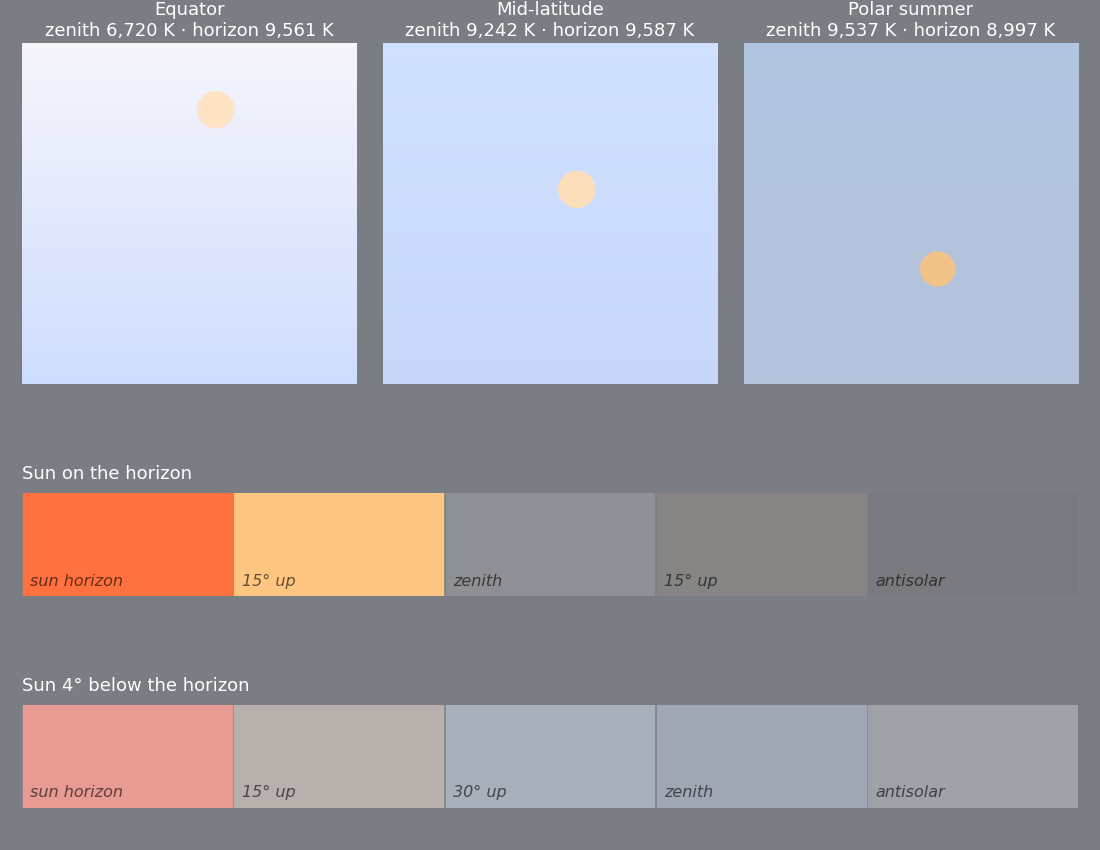
\includegraphics[width=\linewidth]{figures/sky_volcanic.png}
\captionof{figure}{Volcanic year (Tambora 1815 / Toba-lite). Top: noon sky dome at the equator, mid-latitude and polar summer, zenith at top, horizon at bottom, Sun's disk in its own color. Below: sky from the solar horizon to the antisolar horizon with the Sun on the horizon and $4^\circ$ below it.}
\end{minipage}\par\vspace{4pt}
A Tambora-scale sulfate veil ($\tau\approx$0.4) is what most people picture as a spectacular sky, and the model agrees. Noon skies are milky, whiter at the zenith than the horizon (the reverse of a clean sky). Sunsets glow salmon-orange, and the after-sunset sky 15--30$^\circ$ above the horizon turns a luminous pink-lavender: the high sulfate layer is still lit when the lower atmosphere is in shadow. This is the sky of Turner's 1816 paintings and of the Krakatoa twilights of 1883.

\par\vspace{6pt}\noindent\begin{minipage}{\linewidth}
{\normalsize\bfseries Ozone-hole spring\par}
{\small\itshape Antarctic spring in the ozone-hole years: column 130 DU\par}\vspace{3pt}
\centering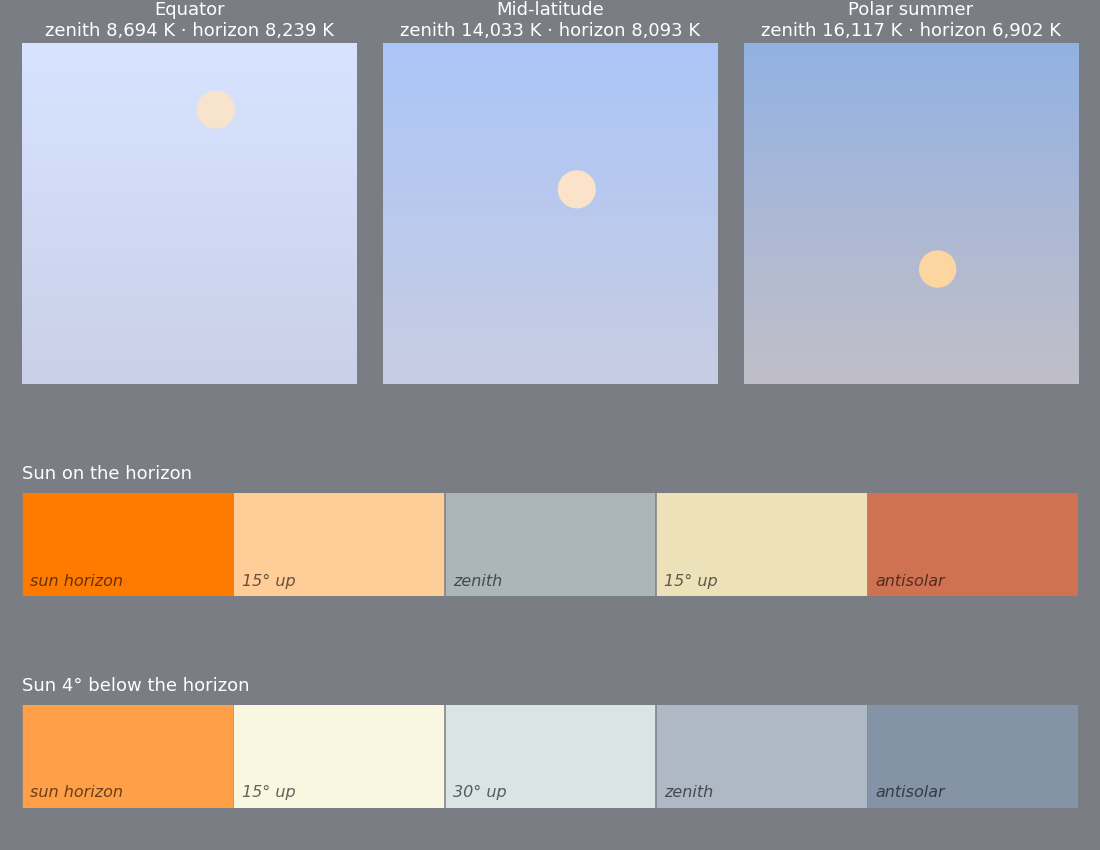
\includegraphics[width=\linewidth]{figures/sky_ozonehole.png}
\captionof{figure}{Ozone-hole spring. Top: noon sky dome at the equator, mid-latitude and polar summer, zenith at top, horizon at bottom, Sun's disk in its own color. Below: sky from the solar horizon to the antisolar horizon with the Sun on the horizon and $4^\circ$ below it.}
\end{minipage}\par\vspace{4pt}
Antarctic spring in the ozone-hole years, with the column cut to 130 DU and the layer lowered toward 18 km. Noon stays blue. Twilight is where the hole shows: with the Sun 4$^\circ$ down the zenith is a pale blue ($\sim$7,800 K) instead of the deep blue ($\sim$12,500 K) of a 300 DU sky. It is the same direction as the thin post-oxidation column, and still well short of the cream ($\sim$6,000 K) of a sky with no ozone at all.

\par\vspace{6pt}\noindent\begin{minipage}{\linewidth}
{\normalsize\bfseries Modern, clean air\par}
{\small\itshape aerosol optical depth 0.1; ozone 260/300/330 DU by latitude\par}\vspace{3pt}
\centering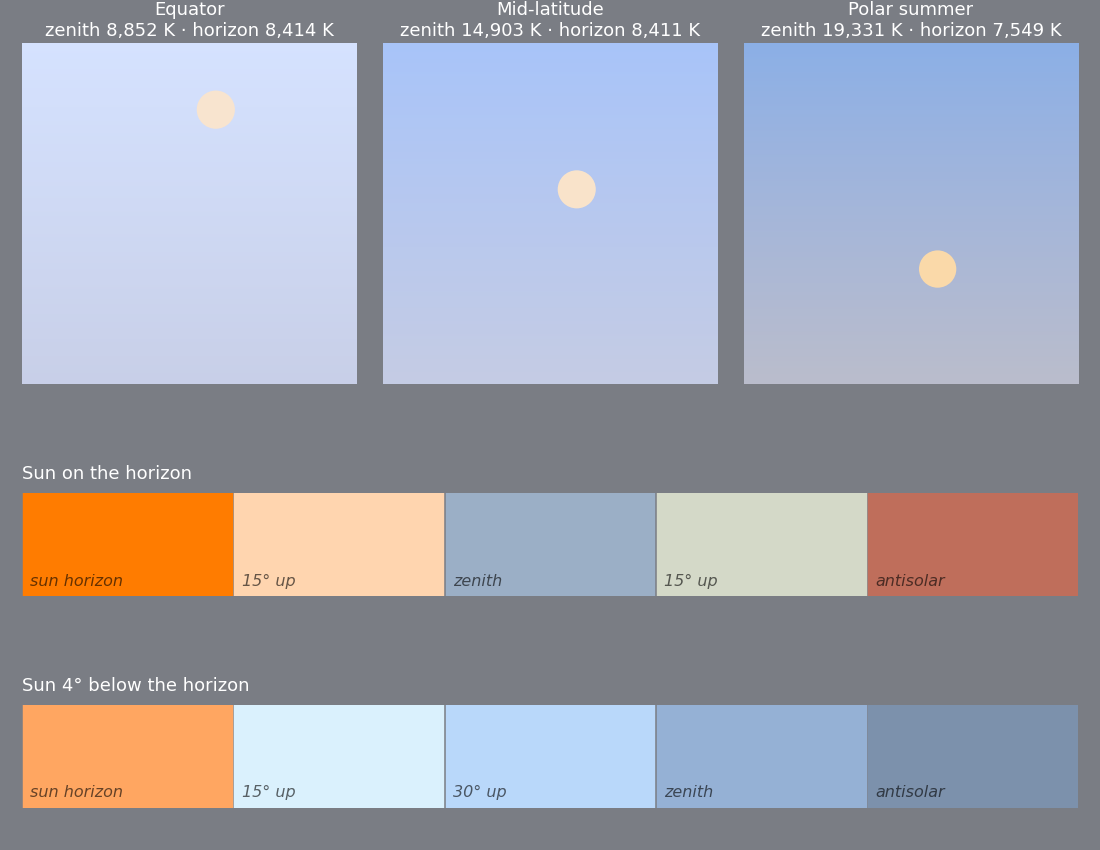
\includegraphics[width=\linewidth]{figures/sky_modern.png}
\captionof{figure}{Modern, clean air. Top: noon sky dome at the equator, mid-latitude and polar summer, zenith at top, horizon at bottom, Sun's disk in its own color. Below: sky from the solar horizon to the antisolar horizon with the Sun on the horizon and $4^\circ$ below it.}
\end{minipage}\par\vspace{4pt}
Baseline. Equatorial zenith $\sim$9,000 K; mid-latitude $\sim$15,000 K; polar summer $\sim$19,000 K. Horizons run 7,400--8,400 K, essentially white. Setting Sun $\sim$1,700 K; solar horizon orange; antisolar horizon pink.

\par\vspace{6pt}\noindent\begin{minipage}{\linewidth}
{\normalsize\bfseries Modern, polluted megacity\par}
{\small\itshape aerosol optical depth 0.6, slightly absorbing\par}\vspace{3pt}
\centering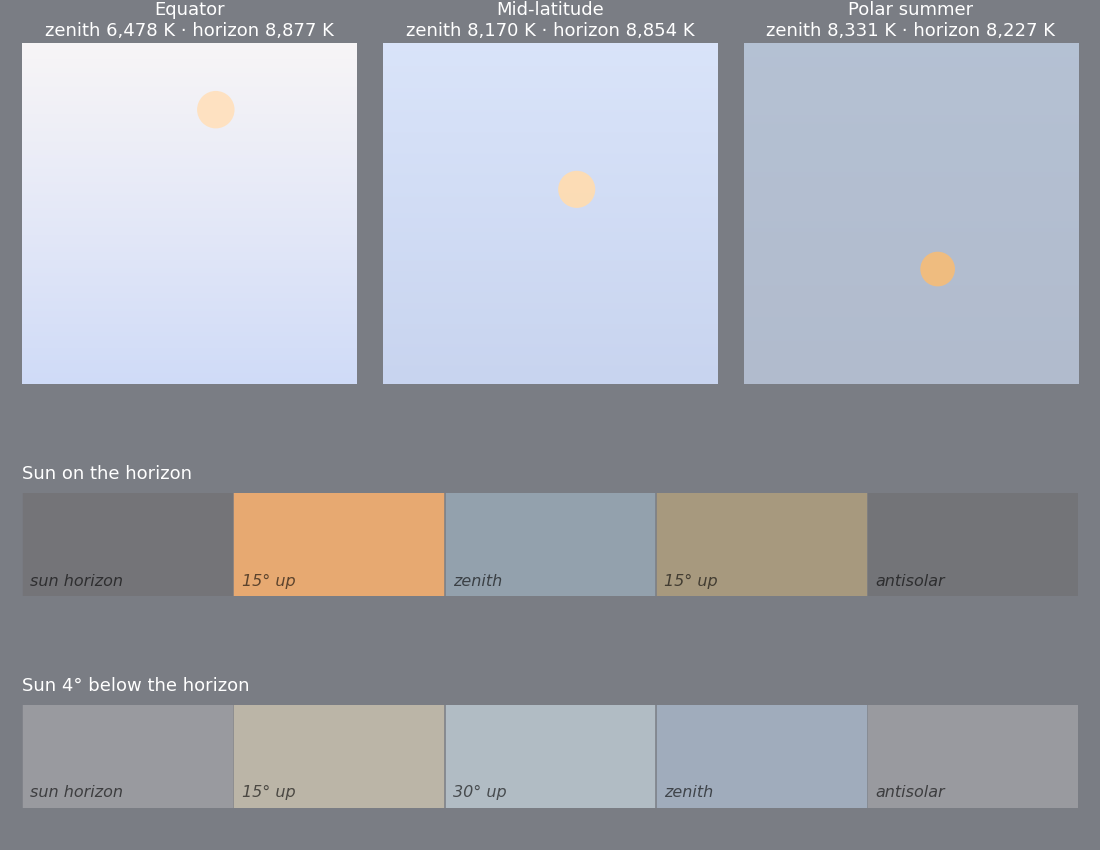
\includegraphics[width=\linewidth]{figures/sky_modernpoll.png}
\captionof{figure}{Modern, polluted megacity. Top: noon sky dome at the equator, mid-latitude and polar summer, zenith at top, horizon at bottom, Sun's disk in its own color. Below: sky from the solar horizon to the antisolar horizon with the Sun on the horizon and $4^\circ$ below it.}
\end{minipage}\par\vspace{4pt}
Aerosol optical depth 0.6 flattens the sky to a near-uniform pale gray-blue (6,500--8,300 K), brighter and whiter at the zenith than a clean sky, with the horizon slightly bluer than the zenith. The Sun disappears into gray murk well before it reaches the horizon.

\par\vspace{6pt}\noindent\begin{minipage}{\linewidth}
{\normalsize\bfseries Year 2100\par}
{\small\itshape today's clean air, with the filed megaconstellation and the Sunrise orbital datacenters\par}\vspace{3pt}
\centering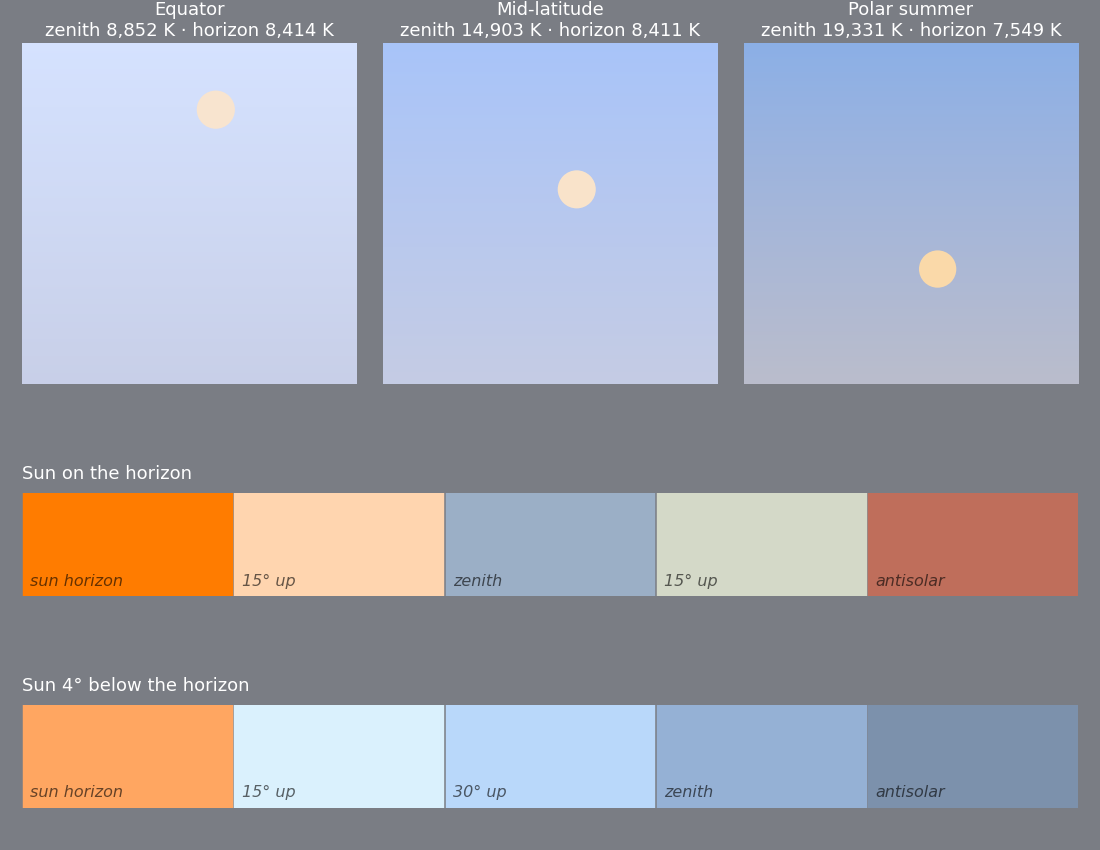
\includegraphics[width=\linewidth]{figures/sky_modern.png}
\captionof{figure}{Year 2100. Top: noon sky dome at the equator, mid-latitude and polar summer, zenith at top, horizon at bottom, Sun's disk in its own color. Below: sky from the solar horizon to the antisolar horizon with the Sun on the horizon and $4^\circ$ below it.}
\end{minipage}\par\vspace{4pt}
The air is today's. What changes is the traffic. Lawler, Boley, and Rein (2022) put every filed megaconstellation on orbit, about 65,000 satellites, and found the worst naked-eye light pollution near 50$^\circ$ latitude. Each of those is their diffuse sphere, effective area 0.8 m$^2$, so its magnitude is on the same scale as the stars. At the equinox a mid-latitude sky has a few hundred of them above naked-eye brightness in the hour after sunset, and Earth's shadow takes them by midnight. On top of that fleet, Boley, Lawler, and Rein (2026) model orbital datacenters. Of the three filed designs, this sky takes the middle one and the more optimistic of their two node spreads: Blue Origin's Sunrise, 51,600 Sun-synchronous satellites from 500 to 1,800 km, in a dawn-dusk cross of rings whose nodes wander 10$^\circ$ to either side of the terminator. Each is a diffuse sphere of 800 m$^2$ at albedo 0.2, the size the paper calls conservative next to panels several times larger, and two hundred times the reflecting area of a communications satellite. An hour after sunset at mid-latitudes, thousands of them are above naked-eye brightness, a bright band along the terminator. The paper's all-night winter rings belong to the December solstice, which this equinox clock does not show. A low orbit crosses the dome in minutes.


\Needspace*{12\baselineskip}
\section*{Beyond the colors}
The colors above are the radiative-transfer model's. The interactive site builds more on the same atmospheres: the setting Sun bent and dimmed band by band, moonlight, solar and lunar eclipses, ice halos, the night sky's own light, aurorae, meteors, and the dust and comets of each era. This part describes each, how it follows the epoch's air, and which numbers are measured and which are estimates. The lunar eclipses are a result in their own right: Earth's transmission spectrum has been computed through geological time as a transiting exoplanet would show it (Kaltenegger, Lin \& Madden 2020), and today's eclipse has been modeled with refraction (García Muñoz et al. 2012), but a search of the Valency corpus finds no reconstruction of how the eclipsed Moon itself looked in past epochs.

\subsection*{The setting Sun}
Near the horizon the Sun is drawn as twenty images, one per 20 nm band from 385 to 765 nm, each lifted by its own refraction (the dispersion of air, Edlén 1966) and dimmed by its own optical depth along the grazing path through the epoch's model atmosphere. At the horizon the green and orange images of today's Sun are only about 6 arcseconds apart, so the colors separate only in the last sliver: the green flash is whichever band survives the extinction last, and the cleaner the air the shorter that wavelength. Along the horizontal path, the model's air still passes a twentieth of its peak sunlight at 550 nm in the clean, dry Snowball epoch, the best flashes in the record, and at 630 nm in today's clean air; under the Neoarchean haze, the impact-winter soot, a volcanic veil or a polluted city nothing shorter than 650 to 730 nm gets through, and there is no flash at all.

How far the air lifts the Sun follows its refractivity, the sum over its gases' partial pressures. Today's horizon refraction of about 34 arcminutes is 1.8 times larger at 4.0 Ga (half a bar of CO$_2$ on a bar of N$_2$), 1.11 times in the oxygen-rich Carboniferous and 0.83 times in Snowball Earth's thinner air, so the Sun sets later or earlier by a minute or two. The 30-bar Hadean air is 47 times as refractive as today's: a horizontal ray bends faster than the ground curves and is trapped (ducting), but its Sun is lost in Rayleigh scattering long before it reaches the horizon, so the drawing holds the bending to three times today's.

Each evening also has its own layering of the low air, set by the date so that a given evening always sets the same way. Thin temperature inversions step the disk's edge, show a strip of it twice (once inverted) where the rays cross, and draw a dark line across it where trapped rays run through the densest air; over warm water the Sun meets its own inverted image in an inferior mirage, the ``omega'' sunset. The cold surface of Snowball Earth makes inversions common and inferior mirages rare, and the warm oceans of the Hadean and Archean the reverse. These mirage statistics are illustrative. The disk is also darker and redder toward its edge (limb darkening, Hestroffer \& Magnan 1998): the air only multiplies the Sun's light, so the darkening is the same under every sky.

\subsection*{Moonlight and the Moon}
Moonlight is the same sky model with the Moon in place of the Sun, scaled by the lunar phase (the Allen phase law with the opposition surge, as in Krisciunas \& Schaefer 1991) and by the inverse square of the Earth--Moon distance, which follows Farhat et al. (2022) back to 2.2 Ga and reaches about 70\% of today's by 3.2 Ga (Eulenfeld \& Heubeck 2023): 47.6 Earth radii at 2.7 Ga and 38.7 at 4.4 Ga. The full Moon was then up to 2.4 times as bright and 1.55 times as wide. Holding the Earth--Moon angular momentum fixed gives days of 23.8 hours at 66 Ma, 17.4 at 2.2 Ga, 15.6 at 2.7 Ga and about 12$\frac{1}{2}$ in the Hadean, matching Farhat et al.; the closer Moon also went round faster, so a month was 20 of today's days at 2.7 Ga and 15 at 4.4 Ga, still 28 to 31 of the shorter days.

The Moon's face changes too. Its dark maria are basalt that flooded the great basins from about 3.9 Ga, most of it by 3.3 Ga (Hiesinger et al. 2011), so each mare is darkened from a date just before its oldest dated basalt: at 3.8 Ga Tranquillitatis is two-thirds dark while Imbrium is still a bright basin, and in the Hadean the near side is bright highland from limb to limb. Tycho's rays, 108 million years old, are missing from the older Moons. Moonlight therefore stays nearly the same in color but not in brightness: a Hadean full Moon lit a 30-bar sky that, like its day sky, was a featureless peach glow.

\subsection*{Solar eclipses}
When the Moon covers part of the Sun, all the sunlit sky dims by the fraction of the disk still showing. In totality the sky is lit from beyond the Moon's shadow, tens to a hundred kilometres away, where the Sun is still partly up: the epoch's own twilight sky with a sunset glow all round the horizon, a thousandth of the day sky, as measured (Sharp, Lloyd \& Silverman 1966; Shaw et al. 2026). The Hadean and hazy Archean totality skies are therefore that era's dusk, peach or amber rather than the deep blue of a modern eclipse.

The corona follows the Sun's age. A younger Sun spun faster and was far more active: its X-ray output goes as age to the $-$1.5 (Güdel, Guinan \& Skinner 1997), about 140 times today's at 4.4 Ga, and its coronal temperature with it, 5 MK against 1.5 MK. Today's corona (Baumbach 1937: electron-scattered K light near the limb, dust-scattered F light beyond about 2.3 solar radii) is scaled accordingly: a denser, more extended K corona, an F corona that follows the era's zodiacal dust, stronger coronal lines (the green Fe XIV and red Fe X, joined by yellow Ca XV in the hot young corona) and a brighter pink chromosphere. These scalings are estimates. The young Sun was also smaller (0.90 of today's radius at 4.4 Ga) while the Moon was closer, so early eclipses hide the inner corona: at 3.8 Ga the Moon looks 1.5 times the Sun's width, and from 2.2 Ga back every central eclipse is total. Through the 30-bar Hadean air, at 7.6 magnitudes of extinction per airmass, the corona does not show at all.

\subsection*{Lunar eclipses}
In a lunar eclipse the Moon passes through the Earth's shadow, which is lit only by sunlight bent into it through the Earth's limb: every sunrise and sunset on Earth at once. Its color and brightness are a measurement of the whole atmosphere at the terminator, which is why eclipses darkened after Tambora, Krakatoa, El Chichón and Pinatubo (Keen 1983; Stothers 2004) and dimmed measurably after the small Kasatochi eruption of 2008 (García Muñoz et al. 2011), and why the eclipsed Moon's spectrum is Earth's transmission spectrum as an exoplanet would show it (Pallé et al. 2009). The same physics, run on each epoch's air, gives the eclipse of every era.

The model (\emph{lunar\_eclipse.py}) traces rays from the Sun through the epoch's atmosphere at tangent heights from the ground to 120 km, bending with the refractivity of its gas mix and accumulating the optical depth of every component (gas, ozone, aerosol, sulfate, haze, soot) along the whole path, with today's cloud tops cutting the lowest rays. Seen from a point on the Moon, the Earth's limb at each position angle and height shows the Sun's limb-darkened disk wherever the ray's bending puts it; summing that over the ring of the limb (Link's method; Link 1969; García Muñoz et al. 2012 for a modern treatment) gives the spectrum of the light at each distance from the shadow's axis, and the direct sunlight past the top of the air gives the penumbra.

Today's umbra comes out a dull copper. A central eclipse puts the Moon 12.3 magnitudes below the full Moon, about V = $-$0.4, in the range observed for clear-air eclipses, with the center darkest and a paler, slightly bluish edge where ozone's Chappuis band removes the orange from the highest rays (the turquoise fringe of eclipse photographs). Before the Great Oxidation there is no ozone and that edge is orange too. A Tambora-sized sulfate veil puts the Moon near V = +11, a surface brightness of 27 mag/arcsec$^2$, far below the night sky: it vanishes, as it did to observers in June 1816 (Stothers 2004). The K--Pg soot and the thick Neoarchean haze remove it entirely; the thin haze leaves a dim brown-red Moon near V = +5.

Two effects are new to the deep past. The closer Moon sat nearer the Earth than the refracted light comes to a focus (about 300,000 km today, past the Moon's 384,000), so the middle of the shadow is reached only by rays skimming the ground and goes dark: at 3.8 Ga the center of the shadow is a hundred million times fainter than its its edge, a dark core in a glowing ring. And the 30-bar Hadean air is so refractive that below about 27 km its rays are trapped and run round the planet, while the upper air bends light strongly enough to fill the whole umbra: the Hadean Moon in totality is an even, deep red, V = $-$1.7 at 38.7 Earth radii.

The shadow's geometry follows the distances and the young Sun's size. The umbra was 3.1 Moon widths across at 4.4 Ga against 2.7 today, and with twice as many full Moons a year, total lunar eclipses came nearly three times as often, while totality itself lasted at most 104 to 109 minutes in every epoch (Table~\ref{tab:lunar}). The rate also depends on the tilt of the Moon's orbit. It was a little steeper then: integrating today's 5.145$^\circ$ back along the distance history with the tidal model of Ćuk et al. (2016), in which Earth's tides flatten the orbit as the Moon recedes and tides raised in the Moon damp it, gives 5.46$^\circ$ at 2.7 Ga and 5.93$^\circ$ at 4.4 Ga (5.8 to 6.3$^\circ$ for a Moon three times stiffer or more dissipative). The much larger tilts that model and Downey, Nimmo \& Matsuyama (2022) need for the young Moon belong to before the Cassini-state transition near 33 Earth radii, older than any epoch here (\emph{lunar\_inclination.py}).

The ephemeris is checked against the almanac. For the total eclipses of 2022, 2025, 2026 and 2029, contact times fall within 2 to 7 minutes of the NASA catalog (Espenak \& Meeus 2009) and umbral magnitudes within 0.04 (for 2029 June 26, 1.831 against 1.844); over 2000--2100 the page finds 144 umbral and 84 total eclipses, against the catalog's 142 and 85. On the page the Moon is drawn for an eye adapted to its brightest part, so the umbra looks black beside the penumbra in a partial phase and glows in totality, as it does to an observer.

\begin{figure*}[t]\centering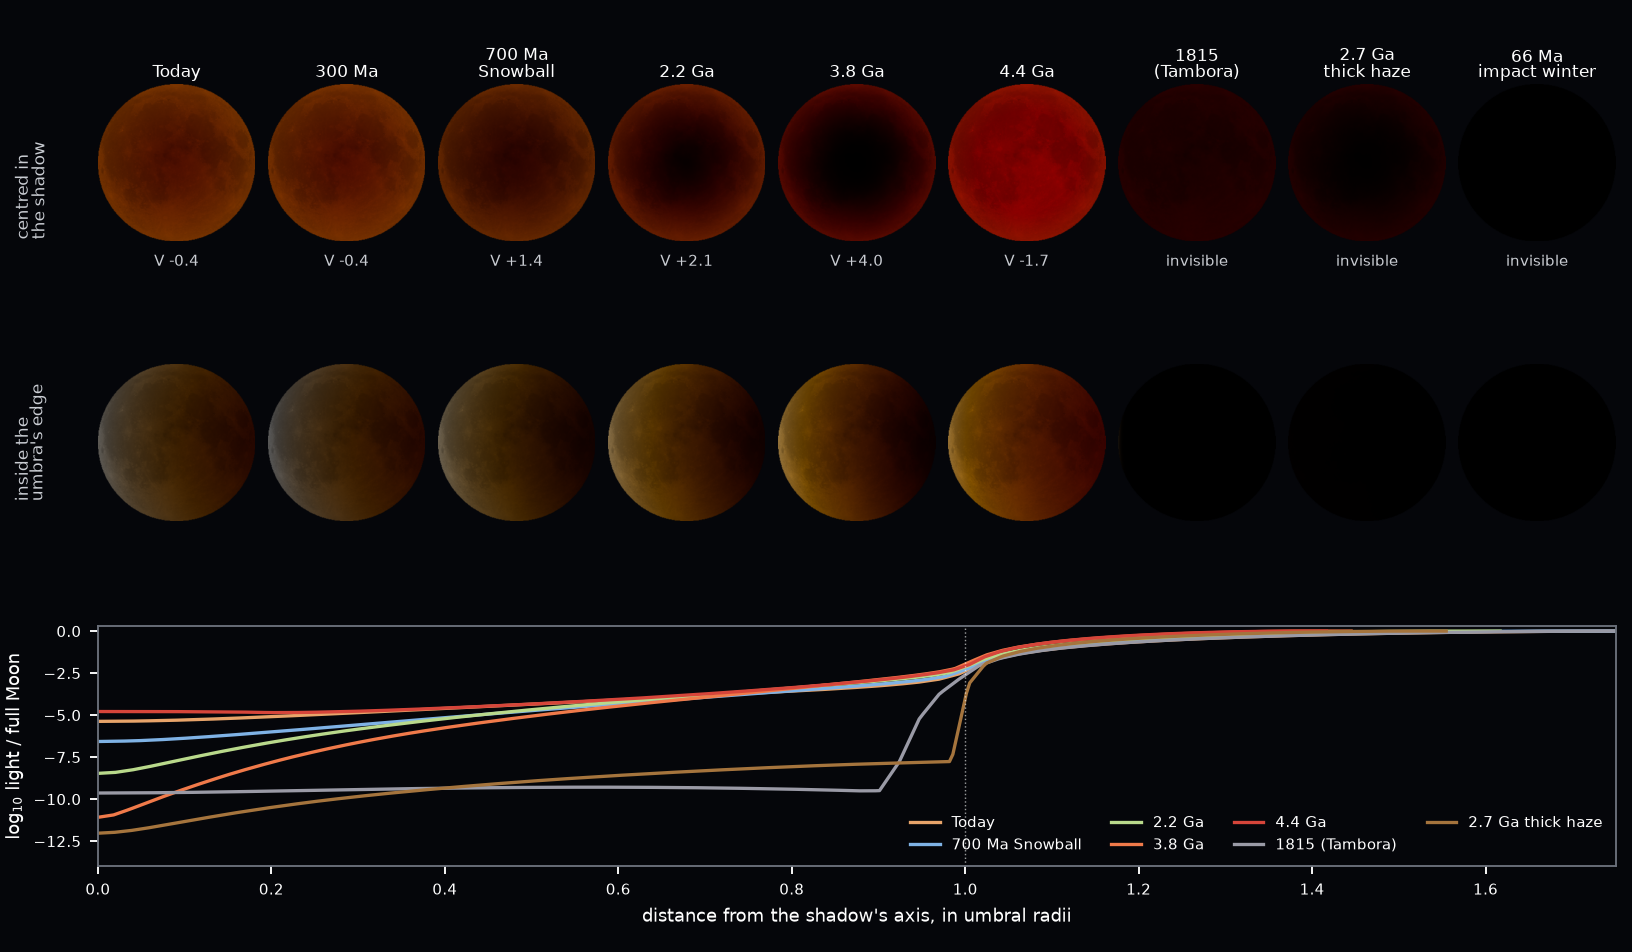
\includegraphics[width=\textwidth]{figures/lunar_eclipse.png}
\caption{The Moon in the Earth's shadow at nine epochs. Top: centered in the shadow, with its V magnitude. Middle: just inside the umbra's edge, where today's ozone leaves a cool gray-blue edge and the ozone-free Archean and Hadean edges are orange. Each Moon is drawn as the page draws it, for an eye adapted to its brightest part, on today's lunar surface. Bottom: the light across the shadow, against the full Moon, with distance in units of each epoch's umbral radius.}\label{fig:lunar}\end{figure*}
\begin{table*}[t]\centering\footnotesize
\caption{Lunar eclipses by epoch. The umbra's diameter is in Moon widths at the mean distance, with Danjon's enlargement. V and the mean surface brightness are for the Moon centered in the shadow, from the model's shadow and the Moon's distance; a dark night sky is about 22 mag/arcsec$^2$. Counts are the page's own over a hundred years of dates (2000--2100), so they carry a few percent of noise from the eclipse cycles. Orbit tilt from lunar\_inclination.py.}\label{tab:lunar}
\rowcolors{2}{rowa}{white}
\begin{tabularx}{\textwidth}{@{}Yrrrrrr@{}}\toprule
Epoch & Umbra (Moon widths) & V at mid-eclipse & Surface brightness (mag/arcsec$^2$) & Orbit tilt & Umbral / total a century & Longest totality (min) \\ \midrule
Today & 2.69 & $-$0.4 & 16 & 5.15$^\circ$ & 144 / 84 & 107 \\
1815 (Tambora) & 2.69 & invisible & 27 & 5.15$^\circ$ & 144 / 84 & 107 \\
66 Ma impact winter & 2.70 & invisible & --- & 5.15$^\circ$ & 149 / 71 & 107 \\
300 Ma & 2.73 & $-$0.4 & 16 & 5.18$^\circ$ & 167 / 76 & 107 \\
466 Ma & 2.74 & +0.3 & 16 & 5.19$^\circ$ & 171 / 74 & 106 \\
700 Ma Snowball & 2.76 & +1.4 & 18 & 5.20$^\circ$ & 172 / 77 & 108 \\
2.2 Ga & 2.90 & +2.1 & 19 & 5.37$^\circ$ & 226 / 124 & 106 \\
2.7 Ga thick haze & 2.96 & invisible & 29 & 5.46$^\circ$ & 286 / 137 & 109 \\
3.8 Ga & 3.09 & +4.0 & 21 & 5.75$^\circ$ & 420 / 211 & 105 \\
4.0 Ga & 3.10 & $-$0.4 & 17 & 5.80$^\circ$ & 438 / 218 & 106 \\
4.4 Ga & 3.12 & $-$1.7 & 15 & 5.93$^\circ$ & 456 / 230 & 104 \\
\bottomrule\end{tabularx}
\end{table*}

\subsection*{Ice halos}
In clear, very cold air the sky fills with diamond dust, tiny hexagonal plates and columns of ice drifting near the ground. Snowball Earth's air would have been full of them at every latitude. Today they are common on the Antarctic plateau and in Arctic winter, so they are drawn at 75$^\circ$ in the modern epochs and in the other cold epochs (2.2 Ga at the end of the Huronian glaciations, the Late Ordovician and Late Paleozoic ice ages, and the Pleistocene), and faintly at 45$^\circ$ at 342 ka, a glacial maximum.

The halos are traced from the crystals' geometry with the refractive index of ice at 450, 550 and 650 nm (Warren \& Brandt 2008), so each arc carries its own dispersion, red toward the Sun: the 22$^\circ$ and 46$^\circ$ halos, the upper and lower tangent arcs, the sun dogs (which move out with the Sun's height and vanish above 61$^\circ$), the circumzenithal arc (only while the Sun is below 32$^\circ$), the parhelic circle with its 120$^\circ$ parhelia, a sun pillar for a low Sun, and the diffraction aureole. The Moon makes the same, faintly. Their brightness, set against the clean noon sky, is an estimate of a good display; the air in front of them is each epoch's.

\subsection*{Twilight and the night sky}
The model is calibrated in absolute units (the clear zenith with the Sun 45$^\circ$ up is 2.7 kcd/m$^2$, which puts the full-Moon sky at the measured 18 mag/arcsec$^2$), so the night can be drawn on the same scale as the day. The sky is computed for Sun heights down to 20$^\circ$ below the horizon; past 9$^\circ$ below, twilight dims by about a magnitude per degree, as measured. Without the Sun or Moon the sky has its own light: today 22.0 mag/arcsec$^2$ at a dark zenith (Leinert et al. 1998), half of it starlight and zodiacal light and half airglow, brighter toward the horizon.

Nearly all of today's airglow needs free oxygen: the 557.7 nm green and 630 nm red lines of oxygen atoms, the hydroxyl bands (H + O$_3$), the sodium D lines cycled through ozone, and the NO$_2$ continuum. It is taken as 90\% of today's at 466 Ma, 80\% in the Snowball epoch (169 DU of ozone and less O$_2$), and 30\% at 2.2 Ga, where 1\% of today's oxygen leaves few atoms near 95 km. Before the Great Oxidation it is gone, replaced by a faint violet glow of the O$_2$ Herzberg II bands from oxygen split off CO$_2$, as on Venus (Krasnopolsky 1983): about as many photons as today's airglow but only 15\% of its luminance, so Archean and Hadean nights were darker and bluer. These strengths are estimates; no model of an anoxic nightglow exists.

Starlight, the Milky Way and the airglow all come from above the air and are dimmed by it: 0.15 magnitude per airmass from the gas plus 1.086 times the epoch's aerosol or haze optical depth, so 0.25 in clean air, 0.8 under the thick haze or a polluted city, 2.3 through the impact-winter soot, and 7.6 under 30 bar of CO$_2$, which hides every star. A star shows only when it is brighter than the naked-eye limit for the sky around it, so stars come out one by one in twilight. The Milky Way is a model in galactic coordinates, peaking at 20.2 mag/arcsec$^2$ in the Sagittarius star cloud, with its center where the Sun's orbit puts it at each age.

In the modern epochs the observer stands in a mid-sized city: a zenith glow of 18.8 mag/arcsec$^2$ today (Falchi et al. 2016), with orange sodium light in 1980--2000 (Cinzano, Falchi \& Elvidge 2001), 1.6 times today's in polluted air, held at today's level in 2100 (the recent 9.6\% a year, Kyba et al. 2023, cannot be projected that far), and almost nothing from the oil lamps of 1815 (Fouquet \& Pearson 2006).

\subsection*{Aurorae}
The aurora is an oval round the magnetic pole, fixed relative to the Sun: on a moderately active night today (Kp 3) it spans about 63--72$^\circ$ latitude on the night side (Feldstein's ovals). Its field lines reach out to the magnetopause, whose distance goes as the sixth root of the field's pressure over the solar wind's. At 3.45 Ga a field half to 70\% of today's and the young Sun's dense wind held the magnetopause at about half today's distance (Tarduno et al. 2010), which brings the oval's edge down to about 50$^\circ$ even in quiet times, and the young Sun's frequent flares and mass ejections (Airapetian et al. 2016) make storms the usual state. Through the Proterozoic the wind weakens (Wood et al. 2005) and the oval retreats toward the pole.

The colors follow the air. Today's green and red lines are oxygen atoms. At 2.2 Ga they are about a third of today's. With no free oxygen the aurora is nitrogen's: violet N$_2^+$ bands and a pink border of N$_2$ first positive bands where faster electrons reach lowest, brighter without oxygen to quench them, with a weak green line from CO$_2$ split by the electrons, as Perseverance saw on Mars (Knutsen et al. 2025). The 30-bar Hadean air is mostly CO$_2$, so there the green line is stronger and the nitrogen faint, though the air hides most of it. Brightness is for a dark-adapted eye, which sees violet far better than the deep red. The ancient line strengths are estimates.

\subsection*{Meteors}
Each meteor is a meteoroid entering the air along a straight path 80 to 125 km up, with its brightness, size and speed tied by the photographic relation of Jacchia, Verniani \& Briggs (1967) and its count set by the measured fireball rate. Today a dark site sees about 8 an hour, more before dawn. A meteor shows only when brighter than the sky around it, so twilight, moonlight and city light thin them out. The air enters three ways. Bright, fast meteors leave persistent trains that glow green and then orange; that chemistry needs oxygen and ozone, so there are no trains before the Great Oxidation. Each meteor's color comes from a spectrum built for its speed and the epoch's air: the metals of the meteoroid, a hotter component that grows with speed, and the air's own emission, oxygen and nitrogen today or carbon monoxide bands in a CO$_2$-rich air, which no one has measured. And in the Early Hadean's 30 bar every density level sits higher, so meteors burn about 22 km higher up.

The rate follows the lunar cratering record (Neukum et al. 2001): about 3,000 times today's at 4.4 Ga, 500 at 4.0 Ga and 120 at 3.8 Ga, of slow, yellow-orange fireballs from a main-belt-like population (Strom et al. 2015; Marchi et al. 2014), with impact flashes on the closer Moon's dark side; twice today's at 2.7 Ga; and a hundred times today's fireballs at 466 Ma, after the L-chondrite parent body broke up (Schmitz et al. 2019).

\subsection*{Dust, comets and the Ordovician ring}
The zodiacal light, sunlight off interplanetary dust, is part of today's natural night sky. Where the inner Solar System held more dust the excess is drawn along the ecliptic, with the gegenschein opposite the Sun: 30 times today's after the L-chondrite break-up and 50 to 1,000 times during the bombardment (estimates after Nesvorný et al. 2010), as bright as a moonlit sky, hiding the fainter stars and meteors. At 466 Ma the speculative debris ring of Tomkins, Martin \& Cawood (2024) is drawn between 1.55 and 2.75 Earth radii with a normal optical depth of at most 0.00015: lost in the blue by day, a low arch at night cut by the Earth's shadow, and at the equator a source of slow, grazing fireballs from the west.

Comets in the modern-era skies are the real ones on their real dates, from JPL's orbits; elsewhere they are drawn at the rate of their time, about one naked-eye comet a year today, 30 times that at 4.4 Ga after the giant planets scattered the comet disk, falling to today's level by about 2 Ga, and 0.6 of today's in the quiet Phanerozoic epochs, since today's sky may still hold the comet shower from the star HD 7977 (Kaib \& Raymond 2026). Their heads and tails are dimmed by each epoch's air like the stars.

\subsection*{Clouds}
Clouds are not part of the radiative-transfer model; the first-person view draws them as scenery, lit by the model's sky. Their regimes are illustrative choices for each era rather than results: a near-overcast stratiform deck under the steamy Hadean CO$_2$, scattered cumulus in the Archean thinning as the haze thickens, sparse thin cloud over the frozen Snowball, towering convection in the warm Carboniferous, almost none in the impact winter, and more cirrus in the volcanic year.

\begin{table*}[t]\centering\footnotesize
\caption{Other phenomena by epoch. Refraction is the horizon bending relative to today's, from the epoch's gases. Airglow and aurora strengths are estimates; the aurora's latitude is the night-side edge of the quiet oval from the magnetopause distance alone (storms, the usual state of the young Sun, push it further toward the equator). Meteor and zodiacal-light rates are relative to today's.}\label{tab:phenomena}
\rowcolors{2}{rowa}{white}
\begin{tabularx}{\textwidth}{@{}lp{2.1cm}YrYrr@{}}\toprule
Epoch & Refraction & Airglow & Starlight extinction (mag/airmass) & Aurora & Meteors & Zodiacal light \\ \midrule
4.4 Ga Hadean & 47$\times$ (trapped) & violet CO$_2$ glow only & 7.6: no stars & oval near 45$^\circ$; green CO$_2$ line, faint N$_2$ & 3,000$\times$ & 1,000$\times$ \\
4.0 Ga Hadean & 1.8$\times$ & violet CO$_2$ glow only & 0.35 & oval near 47$^\circ$; violet and pink N$_2$ & 500$\times$ & 300$\times$ \\
3.8 Ga Archean & 0.97$\times$ & violet CO$_2$ glow only & 0.25 & oval near 50$^\circ$; violet and pink N$_2$ & 120$\times$ & 50$\times$ \\
2.7 Ga Archean & 0.90$\times$ & violet CO$_2$ glow only & 0.25--1.8 with the haze & oval near 54$^\circ$; violet and pink N$_2$ & 2$\times$ & 1.5$\times$ \\
2.2 Ga post-GOE & 0.85$\times$ & oxygen lines at 30\% & 0.25 & oval near 60$^\circ$; O lines at a third & 1.3$\times$ & today \\
700 Ma Snowball & 0.83$\times$ & oxygen lines at 80\% & 0.25 & about today's & 0.6$\times$ & today \\
466 Ma Ordovician & 0.97$\times$ & oxygen lines at 90\% & 0.25 & today's & 100$\times$ fireballs & 30$\times$ \\
300 Ma Carboniferous & 1.11$\times$ & today's & 0.25 & today's & 0.5$\times$ & today \\
66 Ma impact winter & 1.0$\times$ & today's, dimmed by soot & 2.3 & today's & today & today \\
1815 volcanic year & 1.0$\times$ & today's & 0.7 & today's & today & today \\
Today & 1.0$\times$ (34$'$ at the horizon) & 22.0 mag/arcsec$^2$ natural sky & 0.25 & 63--72$^\circ$ at Kp 3; O green and red & 8 an hour & --- \\
\bottomrule\end{tabularx}
\end{table*}


\Needspace*{12\baselineskip}
\section*{Stars brighter than Sirius}
Sirius, at magnitude $-$1.46, is the brightest star in today's night sky, but it has not always been. The Sun's neighbours drift past it at tens of kilometres a second, so a star a hundred parsecs away now may have passed within a few parsecs of it a few million years ago. Tracing every Hipparcos star that has a radial velocity back 10 Myr through the Galaxy, with 2,000 draws over each star's measurement errors, finds eleven that outshone today's Sirius (Table~\ref{tab:encounters}). The brightest is $\theta$ Columbae, a fifth-magnitude star today, which passed about 2 pc from the Sun 4.7 million years ago and peaked near magnitude $-$5, as bright as Venus at its best; Gaia DR3 astrometry gives the same ($-$5.2 at 2.1 pc, 5.1 million years ago). $\varepsilon$ Canis Majoris reached $-$4.35 4.4 million years ago, a result known since \citet{tomkin1998}, and $\beta$ Canis Majoris $-$3.6 at the same time. From about 3.5 to 5 million years ago the night sky held at least two stars brighter than any star today, and at times three.

\begin{table*}[t]\centering\footnotesize
\caption{Stars that outshone today's Sirius ($V=-1.46$) in the last 10 million years, traced back through the Galaxy from Hipparcos astrometry (XHIP) with 2,000 draws over the measurement errors. Peak magnitudes are medians with the 68\% range; the last column is the fraction of draws brighter than Sirius today. Brightness changes with distance only.}
\label{tab:encounters}
\rowcolors{2}{rowa}{white}
\begin{tabularx}{\textwidth}{@{}Yllrrrr@{}}\toprule
Star & Type & Today: $V$, pc & Peak $V$ (68\% range) & Closest (pc) & Myr ago & Brighter than Sirius \\ \midrule
$\theta$ Columbae & B8:IV & $5.00$, 221 & $-5.00$ ($-5.77$ to $-4.41$) & 2.2 & 4.73 & 100\% \\
$\varepsilon$ Canis Majoris (Adara) & B1III & $1.50$, 124 & $-4.35$ ($-4.44$ to $-4.26$) & 8.4 & 4.42 & 100\% \\
$\beta$ Canis Majoris (Mirzam) & B1III & $1.98$, 151 & $-3.58$ ($-3.72$ to $-3.45$) & 11.7 & 4.35 & 100\% \\
$\rho$ Orionis & K0 III & $4.46$, 105 & $-3.16$ ($-4.24$ to $-2.40$) & 3.1 & 2.54 & 100\% \\
Algol & B7V & $2.09$, 28 & $-2.88$ ($-4.65$ to $2.09$) & 2.9 & 5.07 & 62\% \\
$\zeta$ Leporis & A2IV-V(n) & $3.55$, 22 & $-2.54$ ($-2.63$ to $-2.43$) & 1.3 & 0.85 & 100\% \\
$\nu$ Puppis & B7III & $3.17$, 114 & $-2.42$ ($-2.64$ to $-2.22$) & 8.7 & 3.56 & 100\% \\
$\zeta$ Sagittarii (Ascella) & A2.5Va & $2.60$, 27 & $-1.97$ ($-2.07$ to $-1.87$) & 3.3 & 1.05 & 100\% \\
Canopus & A9II & $-0.62$, 95 & $-1.92$ ($-2.01$ to $-1.82$) & 52.2 & 3.18 & 100\% \\
Aldebaran & K5III & $0.87$, 20 & $-1.50$ ($-1.53$ to $-1.47$) & 6.8 & 0.33 & 92\% \\
$\zeta$ Canis Majoris (Furud) & B2.5 V & $3.02$, 111 & $-1.47$ ($-1.87$ to $-0.94$) & 14.0 & 3.27 & 51\% \\
\bottomrule\end{tabularx}
\end{table*}

These stars now lie in Columba, Canis Major and Puppis because that is the solar antapex: the Sun moves toward Hercules at about 20 km/s relative to its neighbours, so the stars it has passed end up behind it. The closest pass, $\zeta$ Leporis at 1.3 pc 850,000 years ago, came as close as $\alpha$ Centauri is now, far too distant to disturb the planets. Only distance changes the brightness here. $\varepsilon$ and $\beta$ Canis Majoris are giants 12 to 22 million years old and were probably a few tenths of a magnitude fainter then. Algol's radial velocity (3.7 $\pm$ 3.9 km/s, hard to measure in an eclipsing binary) is too uncertain to say whether it passed within 1.3 or 28 pc of the Sun. Rigel, Saiph, Mintaka, Alnitak and $\xi$ Persei also come out bright, but 6 to 10 million years ago, about their own ages, so they are left out. The site's skies do not show these peaks: the supernova epochs (1.78 Ma and 342 ka) fall between them, though at 342 ka Aldebaran is close to its peak of $-$1.5.

\section*{Caveats}
Paleoatmospheric compositions carry order-of-magnitude uncertainty, and the haze optical properties are taken from Titan-analog tholins; the three haze cases bracket that uncertainty. Aerosol loads for every pre-Cenozoic epoch are educated guesses. The color-matching functions use an analytic fit, and colors are shown without chromatic adaptation, so the tints represent what a modern camera set to daylight balance would record rather than what an adapted observer would "see" (an adapted eye would perceive the hazy Archean sky as nearer to white and the modern sky as bluer than shown). Clouds are omitted throughout. The two-stream multiple-scattering term is approximate for the thickest atmospheres, where a full Monte Carlo treatment would refine the exact tint of the Hadean sky. Beyond the colors, the strengths of the ancient airglow, aurorae, coronae, meteor and comet rates and zodiacal dust are estimates set to show the trend, as each section says; the lunar eclipses and the orbit's tilt are computed, and the eclipse shadow assumes today's cloud tops in every epoch.

\nocite{*}
\bibliographystyle{plainnat}
% Font expansion fails on the bibliography's small slanted Helvetica, a virtual font.
{\footnotesize\microtypesetup{expansion=false}\bibliography{refs}}

\onecolumn
\section*{Appendix: computed chromaticities}
\scriptsize
\rowcolors{2}{rowa}{white}
\begin{longtable}{@{}llllllr@{}}
\caption{CIE 1931 chromaticity $(x,y)$ and correlated color temperature of the noon zenith and horizon sky, and direct-Sun brightness relative to the modern equatorial Sun. The supernova epochs and the Year 2100 have today's clean air and share its rows.}\\ \toprule
Epoch & Latitude & Zenith $(x,y)$ & CCT (K) & Horizon $(x,y)$ & CCT (K) & Sun \\ \midrule \endfirsthead
\toprule Epoch & Latitude & Zenith $(x,y)$ & CCT (K) & Horizon $(x,y)$ & CCT (K) & Sun \\ \midrule \endhead
Early Hadean, $\sim$4.4 Ga & Equator & 0.421, 0.400 & 3,266 & 0.406, 0.400 & 3,556 & 0.0086 \\
Early Hadean, $\sim$4.4 Ga & Mid-latitude & 0.418, 0.399 & 3,305 & 0.412, 0.400 & 3,443 & 0.0021 \\
Early Hadean, $\sim$4.4 Ga & Polar summer & 0.399, 0.391 & 3,662 & 0.396, 0.392 & 3,719 & 1.4e-06 \\
Late Hadean, $\sim$4.0 Ga & Equator & 0.303, 0.317 & 7,193 & 0.292, 0.302 & 8,328 & 0.63 \\
Late Hadean, $\sim$4.0 Ga & Mid-latitude & 0.275, 0.288 & 10,537 & 0.294, 0.305 & 8,077 & 0.55 \\
Late Hadean, $\sim$4.0 Ga & Polar summer & 0.277, 0.296 & 9,830 & 0.309, 0.320 & 6,795 & 0.25 \\
Early Archean, $\sim$3.8 Ga & Equator & 0.291, 0.303 & 8,340 & 0.299, 0.310 & 7,573 & 0.77 \\
Early Archean, $\sim$3.8 Ga & Mid-latitude & 0.264, 0.274 & 13,112 & 0.301, 0.313 & 7,406 & 0.72 \\
Early Archean, $\sim$3.8 Ga & Polar summer & 0.259, 0.272 & 14,026 & 0.318, 0.330 & 6,207 & 0.47 \\
Neoarchean, $\sim$2.7 Ga (thin haze) & Equator & 0.306, 0.323 & 6,936 & 0.301, 0.316 & 7,325 & 0.72 \\
Neoarchean, $\sim$2.7 Ga (thin haze) & Mid-latitude & 0.288, 0.304 & 8,586 & 0.305, 0.320 & 7,052 & 0.64 \\
Neoarchean, $\sim$2.7 Ga (thin haze) & Polar summer & 0.290, 0.312 & 8,196 & 0.325, 0.340 & 5,829 & 0.31 \\
Neoarchean, $\sim$2.7 Ga (thick haze) & Equator & 0.336, 0.355 & 5,348 & 0.324, 0.346 & 5,858 & 0.46 \\
Neoarchean, $\sim$2.7 Ga (thick haze) & Mid-latitude & 0.331, 0.353 & 5,571 & 0.332, 0.353 & 5,536 & 0.35 \\
Neoarchean, $\sim$2.7 Ga (thick haze) & Polar summer & 0.355, 0.377 & 4,743 & 0.361, 0.379 & 4,573 & 0.07 \\
Neoarchean, $\sim$2.7 Ga (very thick haze) & Equator & 0.386, 0.396 & 3,986 & 0.377, 0.396 & 4,217 & 0.19 \\
Neoarchean, $\sim$2.7 Ga (very thick haze) & Mid-latitude & 0.393, 0.405 & 3,884 & 0.391, 0.406 & 3,943 & 0.1 \\
Neoarchean, $\sim$2.7 Ga (very thick haze) & Polar summer & 0.429, 0.422 & 3,281 & 0.429, 0.423 & 3,289 & 0.004 \\
Paleoproterozoic, $\sim$2.2 Ga & Equator & 0.290, 0.303 & 8,424 & 0.295, 0.306 & 7,928 & 0.87 \\
Paleoproterozoic, $\sim$2.2 Ga & Mid-latitude & 0.264, 0.273 & 13,288 & 0.297, 0.308 & 7,780 & 0.81 \\
Paleoproterozoic, $\sim$2.2 Ga & Polar summer & 0.255, 0.267 & 15,479 & 0.311, 0.323 & 6,643 & 0.51 \\
Snowball Earth, $\sim$700 Ma & Equator & 0.289, 0.297 & 8,737 & 0.278, 0.288 & 10,229 & 0.99 \\
Snowball Earth, $\sim$700 Ma & Mid-latitude & 0.256, 0.262 & 16,181 & 0.282, 0.294 & 9,498 & 0.93 \\
Snowball Earth, $\sim$700 Ma & Polar summer & 0.249, 0.259 & 18,509 & 0.302, 0.319 & 7,234 & 0.62 \\
Ordovician meteor storm, $\sim$466 Ma & Equator & 0.290, 0.302 & 8,425 & 0.291, 0.301 & 8,402 & 0.95 \\
Ordovician meteor storm, $\sim$466 Ma & Mid-latitude & 0.261, 0.269 & 14,206 & 0.291, 0.301 & 8,400 & 0.87 \\
Ordovician meteor storm, $\sim$466 Ma & Polar summer & 0.248, 0.259 & 18,690 & 0.299, 0.310 & 7,593 & 0.5 \\
Carboniferous, $\sim$300 Ma & Equator & 0.290, 0.303 & 8,421 & 0.287, 0.296 & 8,937 & 0.91 \\
Carboniferous, $\sim$300 Ma & Mid-latitude & 0.262, 0.272 & 13,512 & 0.287, 0.296 & 8,930 & 0.82 \\
Carboniferous, $\sim$300 Ma & Polar summer & 0.252, 0.264 & 16,735 & 0.293, 0.302 & 8,178 & 0.41 \\
K-Pg impact winter, 66 Ma & Equator & 0.362, 0.369 & 4,496 & 0.343, 0.353 & 5,096 & 0.12 \\
K-Pg impact winter, 66 Ma & Mid-latitude & 0.360, 0.367 & 4,558 & 0.350, 0.360 & 4,839 & 0.054 \\
K-Pg impact winter, 66 Ma & Polar summer & 0.372, 0.374 & 4,223 & 0.365, 0.369 & 4,401 & 0.00038 \\
Volcanic year (Tambora 1815 / Toba-lite) & Equator & 0.310, 0.324 & 6,720 & 0.282, 0.293 & 9,561 & 0.67 \\
Volcanic year (Tambora 1815 / Toba-lite) & Mid-latitude & 0.283, 0.296 & 9,242 & 0.281, 0.293 & 9,587 & 0.53 \\
Volcanic year (Tambora 1815 / Toba-lite) & Polar summer & 0.280, 0.296 & 9,537 & 0.285, 0.299 & 8,997 & 0.13 \\
Ozone-hole spring & Equator & 0.288, 0.300 & 8,694 & 0.293, 0.303 & 8,239 & 1 \\
Ozone-hole spring & Mid-latitude & 0.261, 0.270 & 14,033 & 0.294, 0.304 & 8,093 & 0.94 \\
Ozone-hole spring & Polar summer & 0.254, 0.265 & 16,117 & 0.307, 0.319 & 6,902 & 0.57 \\
Modern, clean air & Equator & 0.287, 0.299 & 8,852 & 0.291, 0.301 & 8,414 & 1 \\
Modern, clean air & Mid-latitude & 0.259, 0.267 & 14,903 & 0.291, 0.301 & 8,411 & 0.92 \\
Modern, clean air & Polar summer & 0.247, 0.257 & 19,331 & 0.299, 0.310 & 7,549 & 0.53 \\
Modern, polluted megacity & Equator & 0.313, 0.328 & 6,478 & 0.287, 0.298 & 8,877 & 0.6 \\
Modern, polluted megacity & Mid-latitude & 0.292, 0.306 & 8,170 & 0.287, 0.299 & 8,854 & 0.45 \\
Modern, polluted megacity & Polar summer & 0.290, 0.306 & 8,331 & 0.291, 0.306 & 8,227 & 0.08 \\
\bottomrule
\end{longtable}
\end{document}
